\documentclass[thesis_msc.tex]{subfiles}

\begin{document}

\chapter{Introduction} \label{intro}
 
     \paragraph{} In this chapter, the history of pulsars will be briefly discussed. I will describe the formation of pulsars and the models used to describe them. Then, I will introduce the effect of the interstellar medium (ISM) on electromagnetic waves. Applications of pulsars as physics tools will be briefly discussed here. 


    \section{What are Pulsars?}
    \paragraph{} In 1967, Antony Hewish and Jocelyn Bell discovered radio pulsations from the sky with a period of 1.34s \citep{HEWISH1968}. They identified them as an extraterrestrial source because of their fixed position in equatorial coordinates.  After the discoveries of similar sources from the sky, the word ``pulsar " (from pulsating star) is used to describe these objects. The maximum size of pulsar, which is approximated from light travel time across the pulsed emission, \citep{HEWISH1968} must be shorter than light travel time across the object. As a result, the short rotation period of the pulsar leads to the deduction that this object has to be relatively small \footnote{as the period is 1.34s, the maximum diameter of this object should be in the same order as the orbit of the Moon}. Pulsars were hypothesised to be either rotating neutron stars (NS) or white dwarfs (WD). Both NS and WD are remnants of stars which collapsed into compact objects. \cite{PhysRev.46.76.2} proposed the NS theory despite no evidence on this object. After that, \cite{staelin1969passive} discovered the Crab pulsar which  is located in a supernova remnant \textit{Crab nebular}  with a period of 33 ms.  \cite{PACINI1967} and \cite{GOLD1968} confirmed that pulsars are rotating NS because the short period indicates that this object needs to be more massive but smaller than WD (More detailed can be found in \cite{GOLD1968}.   
    %Short period and the location in supernova remnants of the Crab pulsar make us understand that it is associated with NS as it is the last process of an intermediate mass star (See more in Section \ref{formation}) 
               
    \paragraph{} 50 years after the discovery of the first pulsar, the number of confirmed pulsars detected in June 2018 is approximately 2600 \citep{PSRCAT2}. \footnote{The up-to-date number can be found from http://www.atnf.csiro.au/people/pulsar/psrcat.} Some significant milestones of pulsar astronomy are listed below.

\begin{itemize}
\item In 1934 Walter Baade and Fritz Zwicky proposed that dense stars consist of purely neutrons which could be a result from supernovae  \citep{baade1934remarks}.

\item Franco Pacini suggested that neutron stars radiate electromagnetic waves in 1967 \citep{PACINI1967}. 
\item In 1967, the first pulsar was discovered \citep{HEWISH1968}.

\item The discovery of the first pulsar gave  Antony Hewish a share of 1974 Nobel Prize in Physics \citep{HEWISH1968} for his contribution to the discovery of the first NS.

\item Hulse-Taylor pulsar, PSR B1913+16,  was discovered in 1974. This system is the first experimental demonstration of the existence of the Gravitational waves (GW) and earned them the 1993 Nobel Prize in Physics \citep{hulse1975discovery}.

\item The discovery of first pulsar has a rotation period in the order of milliseconds  (B1937+21) with a period of 1.56 ms \citep{backer1982millisecond}. 

\item The first magnetar \citep{kouveliotou1998x} was discovered in 1996. Further detail about magnetars can be found at Section \ref{magnetar}

\item The first ``Double pulsar'' system was discovered in 2003 (\cite{burgay2003increased} and \cite{lyne2004double}). This system  consists of two pulsars. These pulsars allow us to make better constraints on strong-field gravitational theory.


\item The Galactic centre magnetar J1745-2900, which is located near the galactic centre in X-ray, was discovered in 2013 (\cite{kennea2013swift} and \cite{eatough2013strong}). This is the first time that astronomers can probe the environment around the galactic centre with a pulsar.  

\end{itemize}

    \section{Formation of Neutron stars} \label{formation}
    \paragraph{} After stars cannot sustain the balance between inward gravitational force and outward force from radiation pressure originated from internal nuclear fusion, the stars will collapse into one of three kinds of astrophysical objects depending on the initial mass of the star. Low mass stars (M \textless 8 solar mass ($M_\odot$ )) like our sun will collapse to WDs. WDs are compact objects composed of electron-degenerate matter. This matter produces outward force from the Fermi pressure which prevents WDs from collapsing (\cite{chandrasekhar1931maximum} and \cite{d1997evolution}). Massive stars (M $>$ 25 $M_\odot$) will end up as black holes (BH). NSs are remnants of core collapsing of intermediate mass stars (8-25 $M_\odot$). Further details about NS and BH evolution can be found in \cite{heger2003massive}. % s Probably worth just putting 8-25 solar mass in brackets after intermediate mass

    \paragraph{} After an intermediate-mass star converts hydrogen into helium in its core, the thermonuclear fusion process will decrease while the mass of the star remains almost unchanged. The gravitational force makes the helium core contracts until the temperature increases high enough to start helium nuclear fusion. This process continues for the lifetime of the star producing more massive elements and of the region if very stable nuclides binding energy from the left side toward the right side, as shown in Figure \ref{binding} . The last element that intermediate-mass produces from nuclear fusion is iron because it has the highest binding energy, as shown in Figure \ref{binding}. After this point, the star could not further produce energy because the fusion process requires more energy than they can produce \citep{burbidge1957synthesis} and decreases their radiation pressure. The core will collapse while the outer layer is blown away. The remains from this process are called supernova remnants. The process of core contraction makes a supernova explosion (specifically for NS formation, Type II supernova). This collapsed core has mass large enough to overcome electron degeneracy pressure that prevents WD from collapsing. The final stage of core collapsing will convert the iron core into a nuclear matter which mainly consists of neutrons. Further details about NS formation can be found in \cite{cameron1969neutron} and \cite{portegies1998formation}. % s core contracts not contract, more massive elements not element. Actually type 1b and 1c will produce SNRs too as they're core collapse too.

    \begin{figure}[htbp] \centering
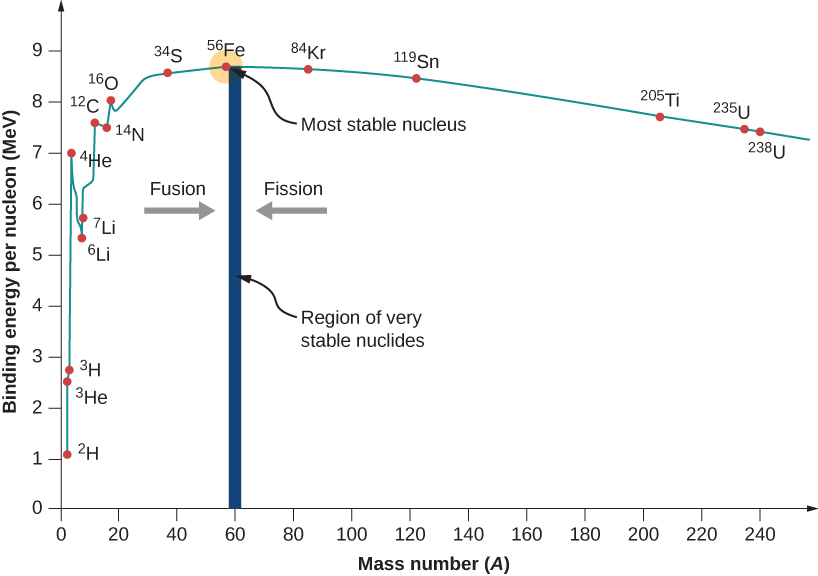
\includegraphics[width=0.70\textwidth]{figures/binding.jpg}
\caption{Relation between binding energy and mass number peaks at iron, which make iron the most stable element. Image from \cite{urone_hinrichs_dirks_sharma_2018} } % s The relation not Relation, peaks not shows peaks

\label{binding}
\end{figure}

\section{Physical model of Neutron stars} \label{phys}
    \paragraph{} The model to describe pulsar emissions is  the \textit{Lighthouse model}. This model describes why pulsar signals are observed as periodic signals by introducing misalignment between the magnetic axis and the rotation axis as Figure \ref{lhmodel}. When a NS spins around the rotation axis, electrons around the magnetic pole of NS are accelerated along the magnetic field line, causing electromagnetic emission. %This emission is parallel with the radio beam produced in Synchrotron process. 
    When the radio beam is pointing towards the Earth, the emission can be observed within the same period as the rotation period. The minimum radius of neutron star with mass $m_p$ and radius R  can be approximated by 

        \begin{equation} \label{rmin}
    R_{min}= \frac{2Gm_p}{c^2}=6.2km \frac{m_p}{1.4M_\odot}
    \end{equation}
Hence, any observable object by electromagnetic radiation needs to be larger than $\frac{3}{2} R_s$ of itself where $R_s$ is the Schwarzschild radius. Otherwise, it will collapse into a black hole. %Check this calculation 
In order to make a stable NS with linear and angular velocity v and $\Omega$  respectively at radius R, the upper limit of NS radius  calculated by considering that NS centrifugal acceleration at the surface needs to be equal to gravitational acceleration. The NS upper radius limit is % s Are you sure it's centrifugal and not centripetal? Centrifugal is an 'inertial force' and is a result of being in a non-inertial reference frame
   \begin{eqnarray}
  %  \frac{v^2}{R}=\frac{Gm_p}{R^2}\\
   % \frac{\Omega^2 R^2}{R}=\frac{Gm_p}{R^2}\\
    R^3=\frac{GM}{\Omega^2}=\frac{Gm_pP^2}{4\pi^2}, 
    \end{eqnarray}
    noted that $\Omega=\frac{2\pi}{P}$, where P is the spin period of NS.
    
    The maximum radius is approximated using
    \begin{equation} \label{rmax}
    R_{max}=(\frac{Gm_pP^2}{4\pi^2})^{\frac{1}{3}}=16.8km (\frac{m_p}{1.4M_\odot})^{\frac{1}{3}}(\frac{P}{ms})^{\frac{2}{3}}.
    \end{equation}
    The canonical mass for NS is 1.4 $M_\odot$ %\citep{stairs2004pulsars} and %
    \citep{antoniadis2016millisecond}. Pulsar mass are measured with the observations of binary neutron stars, as shown in Figure \ref{mass}. The minimum observed period of NS is 1.40 ms \citep{hessels2006radio}. The approximate range of radius of NS is between 10.4 to 12.9 km as reported in \cite{ozel2016masses}. Considering that the moment of inertia that,   
   \begin{equation} \label{I}
   I=km_pR^2
   \end{equation}
assuming that NS is a uniform spherical object (k=0.4), the canonical moment of inertia is $I\simeq 10^{38} kg\cdot m^2$with radius of 10 km and mass of 1.4 $M_\odot$ . 
    \begin{center}
\begin{figure}[h] \centering
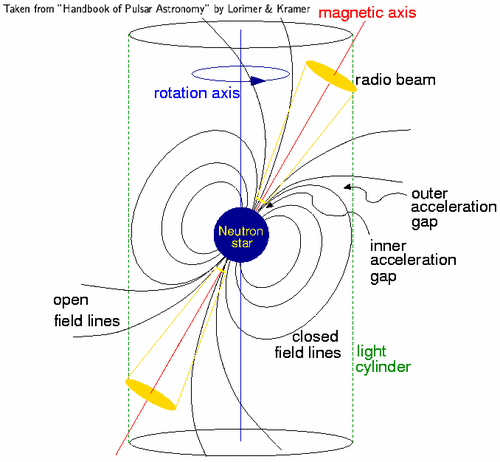
\includegraphics[width=0.7\textwidth]{figures/lhmodel.png}
\caption{Conventional model of a rotating NS (lighthouse model). Image obtained from \citep{handbook}.  }
\label{lhmodel}
\end{figure}
\end{center}   
        \begin{figure}[h!] \centering
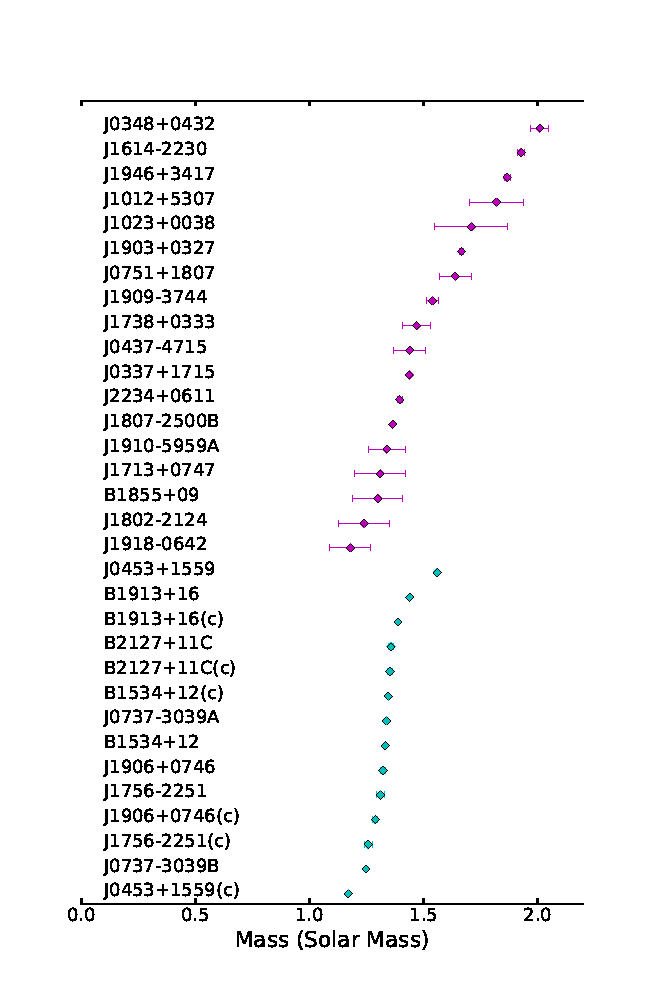
\includegraphics[width=0.6\textwidth]{figures/mass.png}
\caption{The plot of pulsar with known mass with median value around 1.4 $M_\odot$ in line with the canonical mass. Image from \cite{antoniadis2016millisecond}}
\label{mass}
\end{figure}

    \paragraph{} When the core of the progenitor star collapses into a NS due to angular momentum conservation, the rotation period of the NS increases. After that, the spin period increases with time due to energy loss through magnetic dipole radiation process. Giving the rotational energy to be % s Might be worth mentioning as an aside spin-up due to accretion here. 
    \begin{equation}
    E=\frac{1}{2} I \Omega^2.
    \end{equation}
    the energy loss ($\dot{E}$) can be described by 
    \begin{equation}
    \dot{E}=-I\Omega\dot{\Omega}\simeq 3.95\times10^{31}erg s^{-1} (\frac{\dot{P}}{10^{-15}})(\frac{P}{s})^{-3},
    \end{equation}
    where \textit{I} is the moment of inertia. $\Omega$ represents the angular velocity. Assuming that pulsars are similar to spinning magnetic dipoles, the energy loss from  a pulsar with mass $m_p$ and misalignment between magnetic pole to rotation pole $\alpha_i$ is 
   
   \begin{equation} \label{Edotdipole}
   \dot{E}_{dipole}=\frac{2}{3c^3}|m_p|^2\Omega^4 \sin{\alpha_i}^2.
   \end{equation}
   Assuming that all energy loss from a pulsar is magnetic dipole radiation, which gives us 
   \begin{eqnarray} 
   \dot{E}_{dipole}=\dot{E}\\
   \frac{2}{3c^3}|m_p|^2\Omega^4 \sin{\alpha_i}^2=-I\Omega\dot{\Omega}
   \end{eqnarray}
   Then, the relation between $\dot{\Omega}$ and $\Omega$ is
   \begin{equation} \label{omegadot}
   \dot{\Omega}=\frac{2|m_p|^2\sin{\alpha_i}^2}{3Ic^3}\Omega^3.
   \end{equation}
   Equation \ref{omegadot} can be written as $\dot{\Omega}=K\Omega^3$. Using $\Omega=2\pi \nu$, the equation can then be written as 
   \begin{equation} \label{f}
   \dot{\nu}=-K\nu^{n_i}
   \end{equation}
 A braking index ($n_i$) is 3 for the dipole dominated case. However, other sources of energy loss might also affect in this process. Measuring the breaking index allows us to test the energy loss mechanism using only $\nu$ and $\dot{\nu}$. By differentiating Equation \ref{f}.
   \begin{equation} \label{index}
   n_i=\frac{\nu \ddot{\nu}}{\dot{\nu}^2}
   \end{equation}
    $\nu$,$\dot{\nu}$ and $\ddot{\nu}$ are measurable, but only in limited conditions e.g. measuring  $\ddot{\nu}$ is possible only for young pulsars with large $\dot{\nu}$. As a result, a small number of pulsars can measure the braking index. The result from the observation of braking index is between $0.9 \leq n \leq  3.2$ ( \cite{Hamil:2015hqa} and \cite{Archibald:2016hxz}). Wide range of braking index indicates that pulsar energy loss is not dominated only by measuring the magnetic dipole radiation. Moreover, an integration of Equation \ref{f} combined with the fact that $\Omega=\frac{2\pi}{P}$, given that a approximate time from the pulsar at period $P_0$ to decrease to any given $P$ for constant $\dot{P}$ is
    \begin{equation} \label{T}
   T=\frac{P}{(n-1)\dot{P}}[1-\frac{P_0}{P}^{n-1}],
   \end{equation}
   if we assume that the energy loss is purely magnetic dipole (n=3) and $\frac{P_0}{P}<<1$. Equation \ref{T} can be written as  
   
   \begin{equation} \label{tc}
   \tau_c \equiv \frac{P}{2\dot{P}} \simeq 15.8 Myr (\frac{P}{s})(\frac{\dot{P}}{10^{-15}})
   \end{equation}
 $\tau_c$ is defined as characteristic age which gives us an approximate age of a pulsar, again, assuming that there is magnetic dipole. The surface magnetic field is  
    \begin{equation}\label{B}
    B_{surf}=\sqrt[]{\frac{3c^3IP\dot{P}}{8\pi^2R^6sin \alpha_i^2}}.
    \end{equation}
    Using canonical properties of a pulsar with $\alpha$=90, equation \ref{B} can be arranged as
    \begin{equation}
    B_{surf}=3.2\cdot10^{19}\sqrt[]{P\dot{P}} ~ gauss
    \end{equation}
 From this equation, the magnetic field of a pulsar can be calculated simply using only P and $\dot{P}$. From the current pulsar population, the range of $B_{surf}$ is from $10^{11}-10^{14}$ gauss. These values are in line with the measurement from X-ray spectra \citep{coburn2002magnetic}, \citep{bignami2003magnetic}, and \citep{kouveliotou1998x}.  
    
\paragraph{} \cite{conway1962radio} shows that a discrete radio source (later found to be a pulsar) has radio flux distribution that follows power law as $S_{mean} = f^{-a_{obs}}$ with $S_{mean}$ is the mean flux density, $f_{obs}$ is the observing frequency, and $a_{obs}$ is a spectral index with mean value of -1.8 \citep{maron2000pulsar}. This negative spectral index indicates that pulsars are brighter when observed at low frequency.      
   
\section{Pulsar population} \label{pulsartype}
    \paragraph{} The previous section shows that the characteristic age, $\tau_c$, and the surface magnetic field, $B_{surf}$, can be described only with P and $\dot{P}$ in the case of a dipole dominated emission. As a result, one of the most useful tools to study pulsar population is the ``P- $\dot{P}$'' diagram as Figure \ref{ppdot}.  The diagram shows five different types of pulsars: young pulsars, magnetars, ordinary pulsars, mildly recycled pulsars, and recycled pulsars. 
    
        \begin{figure}[h] \centering 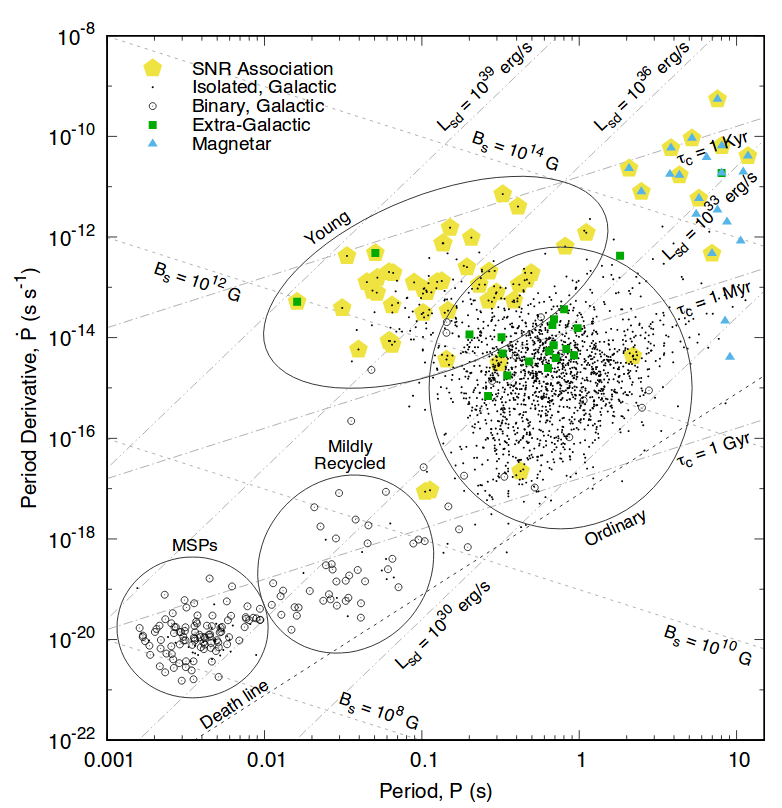
\includegraphics[width=0.7\textwidth]{figures/P-pdot.png}
\caption{ The $P- \dot{P}$ diagram shows five types of pulsars: young pulsars, magnetars,  ordinary pulsars, mildly recycled pulsars, and millisecond pulsars. Quantities, such as $B_{surf}$, $\tau_c$, and $L_{sd}$, are calculated using purely magnetic dipole radiation model.  The death line describes the theoretical region where pulsar's magnetic field can not make radio emission. Figure  is adapted from \cite{Alex}}
\label{ppdot}
\end{figure}

\subsection{Young and Ordinary pulsars}
%%\paragraph{} talk briefly about definition, evolution, missing population as well as SNR timescale.

\paragraph{} A a young pulsar is defined as a pulsar with $\tau_c < 100k$ years. Some young pulsars are associated with SNRs. Young pulsars have relatively wide range of periods from 0.01 s to 1s and $\dot{P}$ greater than $10^{-15}$. Due to the high $\dot{P}$, this type of pulsar has high $\dot{P}$  which means that it is possible to measure $\ddot{P}$ for this pulsar. 
%and $\nu=\frac{1}{P}$
$\ddot{P}$  is important for understanding the radiation process. Young pulsars occasionally \textit{glitch}, meaning that $P$ suddenly decreases. \cite{link1992pulsar} proposed that glitches are an effect of angular momentum transferring inside the NS. Glitches can be used as a probe for NS structure. After a few hundred years, young, energetic pulsars lose their energy and eventually move to the lower right, as shown in Figure \ref{ppdot}. The  largest population in the diagram consists of ordinary pulsars. Ordinary pulsars have a $\tau_c$ range between $10^5 - 10^9$ years. The period is approximately 0.1s to a few seconds. Ordinary pulsars without mass transfer from its companion will lose their energy and end up beyond the  ``death line" \citep{chen1993pulsar}. However, %not all of the pulsars radiate purely magnetic dipole radiation. As a result, 
some pulsars are detectable beyond the death line.  An example of this type of pulsar is PSR J2144-3933 that has a spin period of 8.51s. Detection of pulsar beyond death line indicates the possibility of different radiation processes \citep{zhang2000radio}.        


\subsection{Magnetars} \label{magnetar}

\paragraph{} Magnetars are a group of NS located in the top right part of the ``$P-\dot{P}$" diagram. Magnetars are highly associated with soft gamma ray repeaters powered by their magnetic field \citep{duncan1992formation}. Some magnetars emit electromagnetic waves that more energetic than $\dot{E}_{dipole}$. These objects are called anomalous X-ray pulsars, which imply that magnetars might have different radiation mechanisms. Magnetar's spin periods are ranging between $\sim$ 2 to 12s with high spin down rate ($10^{-15}-10^{-9}$). High spin down rate implies that this type of object have a high $B_{surf}$. This is the reason why this type of object is called ``magnetar''. The slow period and high spin down imply a short life before it crosses the death line in $P-\dot{P}$ diagram.  Some magnetars are not observable at radio frequencies and are known as radio quiet  magnetars. To date, there are only 29 magnetars discovered so far \citep{Olausen:2013bpa}.


\subsection{Mildly recycled and Recycled pulsars}

\begin{figure}[h] \centering 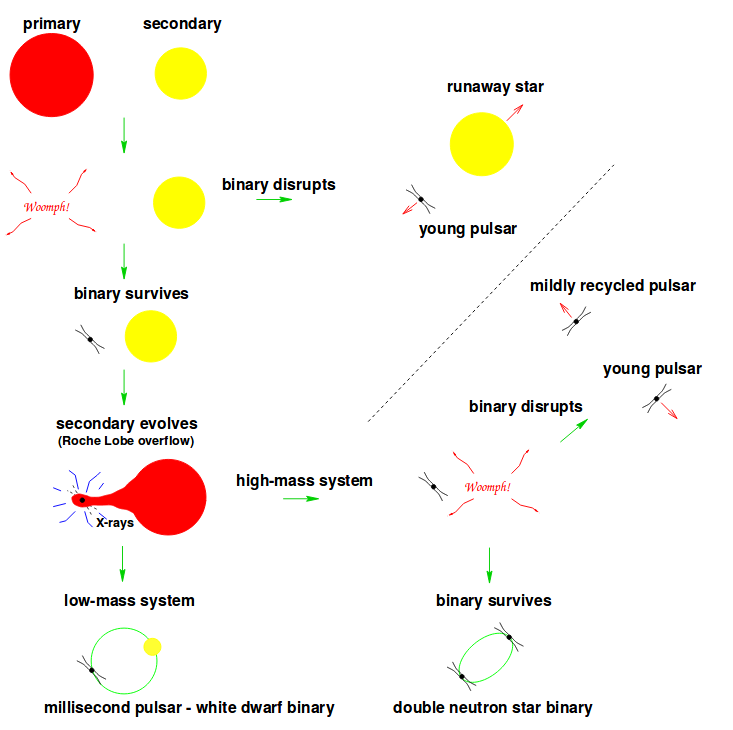
\includegraphics[width=0.75\textwidth]{figures/evo.png}
\caption{Theory of pulsar evolution in a binary system throughout their lifetime. For a binary system with a high mass star, after the life of a higher mass star ends, it will turn into a supernova. If the companion could not survive this process, it will be dispatched with large proper motion. However, this system still can evolve if it can survive this process until the life of the companion star ends. In the case of a low mass companion star, the supernova at the end of its life might not have enough energy to destroy the system. The result from this process is a circular orbital system between NS and WD. In the case of a high mass companion, the supernova at the end of its life is enough to change the orbit eccentricity. If the system can survive, the result of this process is a highly eccentric system of double pulsars. However, if the system could not survive the supernova, the resulting system is a high proper motion mildly recycled pulsar from the first pulsar and a young pulsar from the companion.   }

\label{evo}
\end{figure}

\paragraph{} Ordinary pulsars interact with companion stars through mass transferring.  The angular momentum transfer is making them spinning faster. As shown in Figure \ref{ppdot}, ``faster" pulsars, including recycled pulsars and mildly recycled pulsars, are mostly associated with binary systems. This process will make pulsar moves to the lower left side of the $P-\dot{P}$ diagram while losing their surface magnetic field by mass transferring. This results in a fast pulsar with a period between 0.01-0.2 s but with low $\dot{P} \sim 10^{-18}$ known as recycled pulsars. In this thesis, I will refer to pulsars that spin faster than 20 ms as ``millisecond pulsars''. Recycled pulsars also have the smallest spin down rate because these pulsars have low-surface magnetic fields, making their periods highly stable. Stable period, as a characteristic of recycled pulsars, allows for application of precise time measurement.  

 \section{How do pulsar signals propagate ?}
 \paragraph{} After a pulsar emits a signal, it will travel throughout the ISM, introducing some propagation effects. Two major effects are dispersion and scattering, which will be discussed in this section.   
    \subsection{Pulse dispersion} \label{Pulse_dispersion}
\paragraph{} Because it has been travelling through the Galaxy, the emission from pulsars experiences different wave group velocities, depending on the frequency. The Refractive Index ($\mu_i$) describes the group velocity of electromagnetic waves in different mediums. This is described as equation \ref{rindex}, 
\begin{equation}\label{rindex}
\mu_i=\sqrt{(1-\dfrac{\nu_p}{f})}=\dfrac{v_g}{c},
\end{equation} 
where $f$ is the wave frequency, $\nu_p$ is the plasma frequency, $v_g$ is the group velocity, and $c$ is a speed of light. The Plasma frequency $\nu_p$ can be written as %equation \ref{fp},
 \begin{equation}\label{fp}
 \nu_p=\sqrt{\dfrac{e^2n_e}{\pi m_e}},
  \end{equation} 
with $n_e$, $e$ and $m_e$ are electron density, charge, and electron mass respectively. The light travel time along the length L can be calculated from an integral of  
\begin{equation}\label{lighttraveltime}
 t=\int_{0}^{L}\dfrac{dl}{v_g}=\dfrac{L}{c}+\dfrac{e^2 \int_{0}^{L} n_e dl}{2\pi m_e c f^2}.
\end{equation} 
The first term describes the light travel time in vacuum, while the second term describes the delay caused by frequency dependent refractive index. To simplify this equation, the dispersion measure ($DM$) is defined as  
\begin{equation}
\label{DMdef}
DM=\int_{0}^{L} n_e dl,
\end{equation}
The time delay part from Equation \ref{lighttraveltime} can be re-written as    
\begin{equation}
\label{delaytime}
t=\dfrac{e^2}{2 \pi m_e c }\dfrac{DM}{f^2}=4.15\cdot 10^6 \dfrac{DM}{f^2}\,s.
\end{equation}
The DM is expressed in $pc~cm^{-3}$ \footnote{Parsec ($pc$) is a unit used to describes length in astronomy. (1 pc=$3.1^{15}$ m)  } and $f$ is in MHz. The effect on the time delay is observable only if the radiation is not continuous. From Equation \ref{delaytime}, the DM is estimated from 
\begin{equation}
\label{DMcal}
DM=\dfrac{\Delta t}{4.150\cdot 10^6}(f_{ref}^{-2}-f_{chan}^{-2}) pc ~ cm^{-3}.
\end{equation}
  $\Delta t$ is the difference of time delay between reference frequency ($f_{ref}$) and channel frequency ($f_{chan}$). The example of this effect on pulsar is shown in Figure \ref{DMplot}. Equation \ref{delaytime} shows that this effect would be small for high frequency observation. This effect will smear out the signal, causing difficulty for detecting pulsars at high DM. The way to correct this effect will be discussed in Section \ref{DDM}.    
\begin{figure}[h] \centering
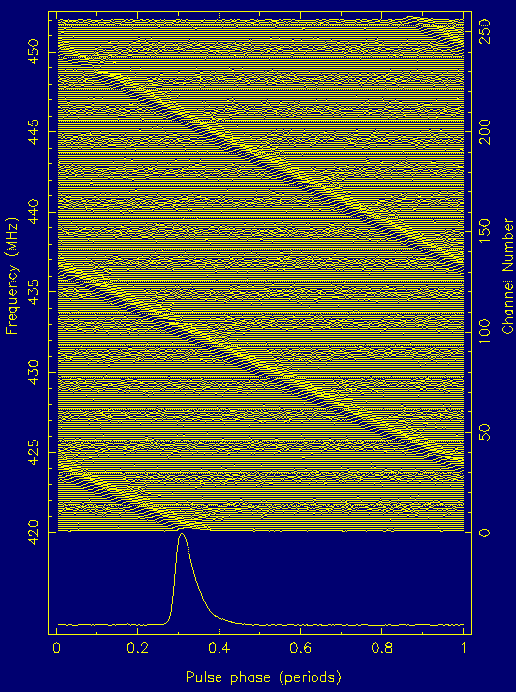
\includegraphics[width=0.5\textwidth]{figures/disp.png}
\caption{Effect of dispersion on a pulse of a pulsar. This effect makes lower frequency data arrives later than high frequency data. Image obtain from http://www.jb.man.ac.uk/distance/frontiers/pulsars/section4.html.  }
\label{DMplot}
\end{figure}
   \paragraph{} The DM represents the number density of electrons along the line of sight to the source, as shown in Equation \ref{delaytime}. The simplest way to describe an electron density distribution in the Galaxy is to imagine it to be uniformly distributed. The typical value for $n_e$ in our Galaxy is 0.03 $cm^{-3}$ \citep{ables1976hydrogen}. However, our Galaxy is much more complicated than the uniform distribution. By taking in account of the shape of the Galaxy and carefully measuring the distance from many pulsars to the Earth, a model for the free electron distribution can be described as \citep{cordes2003ne2001} and \citep{yao2017new} , as shown in Figure \ref{nedist}.  The electron distribution can be used to estimate the distance to the source if we know the density distribution. On the other hand, if the distance to pulsars is measured by other methods, the electron density can be decided. 
   
   %As a result, DM can be used as a probe to measure the distribution of free electrons in the universe as well as the distance between a pulsar to the Earth.     
\begin{figure}[h]
\centering
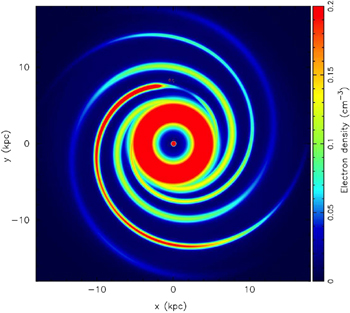
\includegraphics[width=0.5\textwidth]{figures/nedist.jpg}
\caption{Simulated electrons density distribution in the Milky Way galaxy show the spiral structure of our galaxy from the YMW16 model. Image obtained from \citep{yao2017new}  }
\label{nedist}
\end{figure}

    
    \subsection{Pulse scattering}
\paragraph{} When coherent electromagnetic waves from pulsars propagate through the ISM, it changes the signal's path length depending on the frequency. This effect makes an offset in the pulse phase, creating phase delay as shown in Figure \ref{scatt}. This results in a broader pulse profile with an exponential decay tail. This effect is called scattering. 

 \begin{figure}[h] \centering 
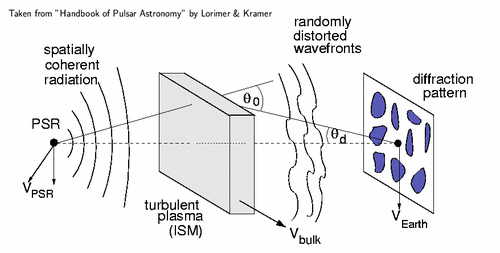
\includegraphics[width=0.8\textwidth]{figures/scatt.png}
\caption{A coherence signal from pulsar being perturbed by ISM, causing an incoherence phase or pulse broadening. Image obtained from \citep{handbook}  }

\label{scatt}
\end{figure}

The exponential decay is defined as $I=I_0 e^{\frac{-t}{\tau_s}}$ , where $\tau_s$ is defined as the scattering time. $\tau_s$ can be measured by deconvolution of the pulse profile with an exponentially decaying function. In the case of the thin screen, it predicts $\tau_s \propto f^{-4}$ \citep{xu2017scatter}. In this case, a pulse from the pulsar is expected to be boarder in the low frequency which reduces the height of the peak as shown in Figure \ref{pscatt}. As a result, this effect can be reduced by observing at higher frequency.

    \begin{figure}[h] \centering 
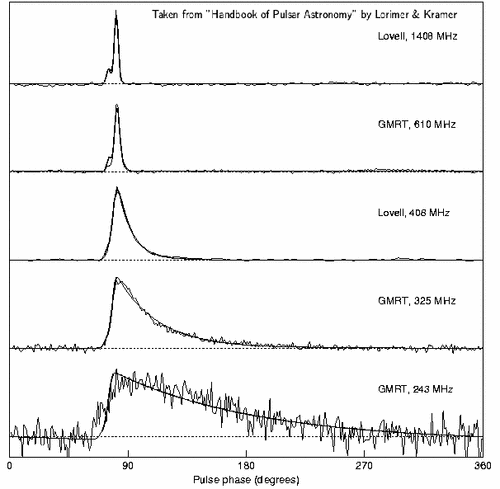
\includegraphics[width=0.5\textwidth]{figures/pulsescat.png}
\caption{Pulse profile from the same pulsar observed at different frequencies showing the exponential decay tail. The effect is increased at low frequencies, making the pulsar harder to detect. \citep{handbook}  }
\label{pscatt}
\end{figure}

\paragraph{} Since both dispersion and scattering are originated from the ISM, they are expected to be correlated. This correlation is shown by \cite{Bhat:2004xt}. The correlation between DM and $\tau_s$ is shown in Figure \ref{t_dm}. Consequentially, pulsars in a high DM environment such as at the centre of the Galaxy are expected to have boarder pulses.  

    \begin{figure}[h] \centering
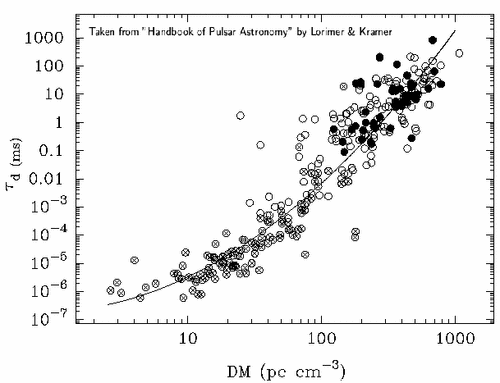
\includegraphics[width=0.5\textwidth]{figures/t_dm.png}
\caption{Correlation between DM and $\tau_s$. Image from \citep{handbook}  }
\label{t_dm}
\end{figure}

\section{Pulsars as physics tools}
    \paragraph{} Pulsars can be used as tools for studying many aspects of physics % e.g. an array of pulsars can be used as a tool for detection of nano-hertz gravitational wave \citep{doi:10.1093/mnras/stw347}.
    The following subsections demonstrate some ways to use pulsar as physics tools.  

    \subsection{Stellar and Pulsar population} 
    \paragraph{} The current pulsar population is biased due to selection effects from the observation sensitivity, either making the location of the pulsars far away from the Earth or weak pulsars harder to detect as shown in Figure \ref{pdist}. As a result, finding more pulsars as many as we can would help us to get a better understanding in our theory of pulsars formation and their progenitor stars. The better understanding of the theory of pulsar formation leads to many applications such as predicting the rate of NS merger. NS merger event estimation is essential for understanding the creation of heavy elements such as gold in our Galaxy \citep{Thielemann:2017acv} and the expected number observable gravitational waves \citep{0034-4885-72-7-076901}.
        \begin{figure}[h] \centering
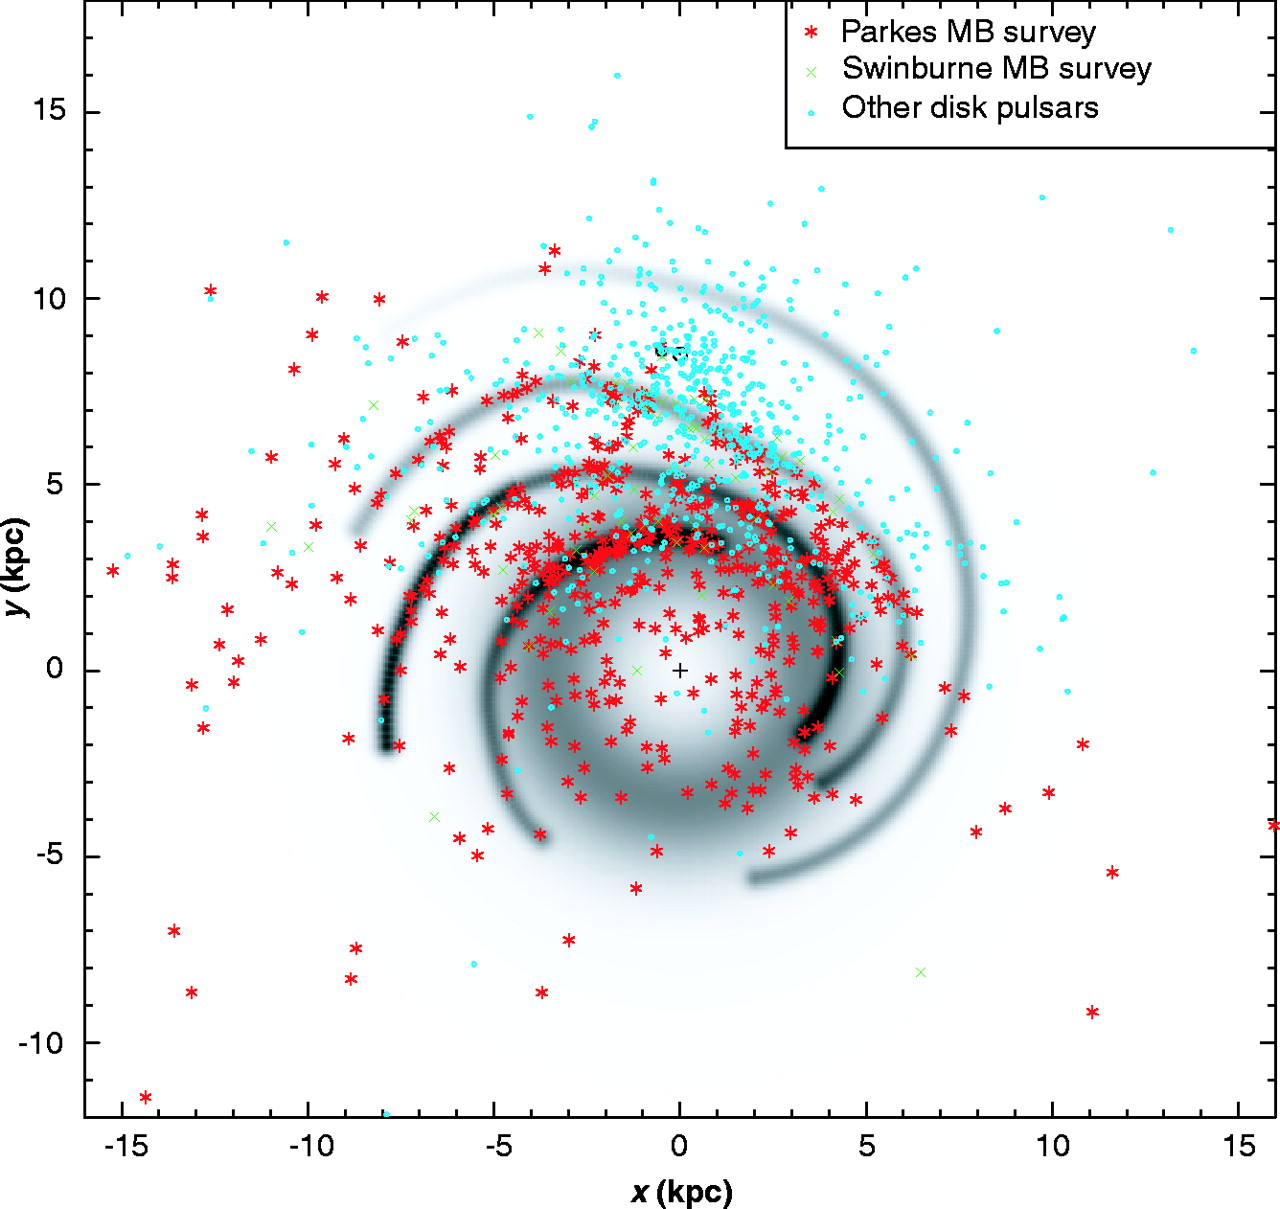
\includegraphics[width=0.4\textwidth]{figures/F1_large.jpg}
\caption{The distribution of pulsars in our Galaxy shows observational bias of pulsar survey on sensitivity. Image obtained from \citep{Manchester542}  }
\label{pdist}
\end{figure}
    \subsection{ISM distribution in the Galaxy}
    \paragraph{} As mentioned in Section \ref{Pulse_dispersion}, studying pulsars gives us information about our Galaxy's ISM distribution. Pulsars are born in supernova explosions. It kicks pulsars out of the Galactic plane, making them well distributed in all directions from the Earth. Widely distributed properties can be used to study our Galaxy in 3D. As a result, pulsars can be an effective probe of the Galactic electron distribution. This already has led to the model of our Galaxy's free electron distribution. Moreover, pulsars can be used to study large-scale structure of Galaxy magnetic field by studying the relationship between DM and effect of Faraday rotation\citep{doi:10.1111/j.1365-2966.2008.13188.x}. 
    
    \subsection{Physics in extreme gravitational field}
    \paragraph{} Pulsars are dense objects which have a strong gravitational field that are impossible to create on the Earth. As a result, pulsars can be used to test general relativity and modified gravity theories. For example, a double neutron star system PSR B1913+16 gives the first detection of gravitational wave radiation as general relativity (GR) predicted that the orbit will change by a centimetre per day \citep{weisberg2004relativistic}. Moreover, the double pulsar system is used to test five separated GR predictions with the uncertainties of $\sim$ 0.05  \%  \citep{kramer2006tests}.  
    \paragraph{} Not only double pulsar systems but also other types of pulsar-binary can be used as physics tools. For example, NS-WD binaries are used as tools for testing the strong equivalence principle \citep{zhu2018tests} as well as the universality of free falling \citep{PhysRevLett.120.241104}. An NS-BH binary system, which still has  not yet been discovered, will also be an excellent tool for testing the strong equivalence principle in a stronger field than NS-NS system. 
        
  % \paragraph{} The Event-Horizon-Telescope Collaboration (EHTC) is aiming to image a shadow of the supermassive black hole at the centre of our Galaxy (Sgr A*). However, \cite{mizuno2018current} suggests that only an image is not able to distinguish between the predicted result from GR and alternative theory. One of the suggestions is to find a pulsar that orbiting around Sgr A* and combine it with the image.      
  
   \subsection{Physics of super-dense matter}
    \paragraph{} Pulsars are super dense objects which are not possible to be produced on the Earth. Binary pulsars are one of the best tools for studying the dense matter. For example, each equation of state predicts different maximum and minimum pulsar masses and radius. %Moreover, glitches can also be used as a tool for study moment of inertial of neutron stars \citep{link1992pulsar}. 
    Some potential equations of state can be ruled out \citep{ozel2016masses} by measuring the mass of a pulsar in binary system period or Shapiro delay.  

\section{Thesis outline}
    \paragraph{} Methods for pulsar searches will be introduced in Chapter \ref{Methods}. This chapter is about the different methods to find pulsars, advantages and disadvantages of each method. Also, I will discuss about the method for binary pulsar searching and how to get rid of radio interference (RFI) as well as a method for de-dispersion.
    %\paragraph{} Chapter \ref{RFI} 
    
    \paragraph{} Introduction various pulsar surveys will be discuss from the beginning of the pulsar survey to current status. After that detailed about the implementation of acceleration search in FFA pipeline will be discussed in Chapter \ref{Chapter:FFA_c}. 
    
    \paragraph{} In Chapter ~\ref{Chapter:result}, results of pulsar discoveries and confirmations from the Fast Folding Algorithm (FFA) pipeline with acceleration search in will be discussed. 
    
    \paragraph{} In chapter \ref{Con}, I will talk about overall conclusions of this work. Also, I will talk about future plan and give the final answer of the question that ``How to finding the slowest pulsars''  
    
\chapter{Methods for pulsar searching} \label{Methods}
\paragraph{} After signals from a pulsar passes throughout the ISM and reaches the radio telescope, the telescope's system will convert this analogue signal to digital signal, which is ready to be processed. In order to detect weak pulses/pulse from a pulsar, three different techniques are used. In this chapter, I will explain about the fast Fourier transform (FFT), the fast folding algorithm (FFA), and single pulse search. However, if this pulsar is in binary or more complex system, signals from this pulsar will suffer from a Doppler shift, changing the apparent period and reducing S/N. The method to prepare the data and mitigate radio frequency interference (RFI) and de-dispersion will also be discussed here. 
    \section{Data acquisition}
		%\paragraph{} Dish collects the radiation from the source. Amplified and down convert by fronted. Convert from AC/DC by backed.  
		\paragraph{} After the signal reaches the telescope, the dish will focus the signal into the primary focal plane. Because the signal from a pulsar is typically weak, the collecting area needs to be large. Examples of telescopes that are used for pulsar observation are the 64-m Parkes radio telescope in Australia, the 100-m Green Bank telescope in the US, the 300-m Arecibo telescope in Puerto Rico, and the 100-m Effelsberg telescope. The equation used to describe the effect of the different dish size on the angular resolution is
        \begin{equation} \label{angular_res}
        \Theta \sim \frac{c}{D \times f_{obs}}, 
        \end{equation}
where c is the speed of light, D is the diameter, and $f_{obs}$ is the observing frequency. Noted that, this equation is valid only in far field case.
        \paragraph{} At the focal plane, the receiver will amplify the signal as soon as possible. Then, the bandpass filter will filter only the selected band of radio frequency (RF). In order to reduce signal loss, the mixer attached with a local oscillator (LO) will down convert the RF to lower intermediate frequency. This part called Fronted. 
		\paragraph{} The backend is where the data get digitised from analogue to digital data. Digitised data will be analysed. %In this work, only the pulsar search backend will be mentioned. 
		In a pulsar search backend, the digitised data will be streamed to the Field Programmable Gate Array (FPGA), which will perform polyphase filterbank with the Fast Fourier transforms (see more in Section \ref{FFT}) to channelise the signal into many individual narrow frequency channels. This data will be stored with the two polarisations summed and be ready to be processed.  
            \section{Data preparations} 
            \paragraph{} After the data is passing throughout backend system, the data is processed in order to detect the weak signals from the pulsar. First, we need to mitigate the radio frequency interference (RFI). Then, we remove the effects of the ISM as aforementioned in Section \ref{Pulse_dispersion}.    
            
   \subsection{RFI mitigation} \label{RFI_mit}
        \paragraph{} RFI decreases the detectability of the pulsar. A strong RFI reduces the sensitivity of the instrument by decreasing the dynamical range and creates artificial pulsar candidates in the pulsar search pipeline. So, one of the first steps of the pulsar search pipeline is to detect and remove strong RFI. 
        
        \paragraph{} There are many approaches of RFI removal. The simplest way is to search for a strong signal in time and frequency domains and filter it out. However, this method might fail to distinguish between a bright transient and a bright pulsar with RFI. Another way is to use the fact that RFI, generated from the Earth, will not suffer from dispersion and appears as zero DM signal. As a result, this type of RFI is removed by filtering out the signal with zero DM. However, this method might affect the detectability of a pulsar with a long period because long period pulsars have a broad DM-curve (a relation between S/N and DM), as mentioned in Section \ref{DDM}. So, the pipeline might mistakenly detect a long period pulsar as a RFI. 
        
        \paragraph{} \cite{Ng} suggested that disadvantages from these methods is compromised by comparing the candidate with other beams from the same observation. Since pulsars are located far from the Earth and relatively weak (0.1 Jy \footnote{The jansky (Jy) is a unit of spectral flux density. (1 Jy = $10^{-26}$ Watt/$m^2$/Hz)}), they are likely to be detected in only one observation beam. On the other hand, RFIs are originated from the Earth and likely to be detected in more than one beam. As a result, the FRI is flagged by comparing the zero-DM Fourier spectrum with all of the observation beams and search for Fourier bins that has $S/N$ exceeds the $S/N_{min}$ in more than four beams and flagging them as periodic RFI.     

     \paragraph{} Another method is to create the list of period bins, which are contaminated by RFI or the ``zap table''. The zap table is also called as the Birdie list. If the zap table is available before searching, period bins in zap table can be flagged by flagging out corresponding period. The flagging is done by applying the FFT to a time series and then zapping out the contaminated Fourier bins. Then, the transformed time series is applied by the inverted FFT, which transforms the Fourier spectrum back to the time series. Results from this process are flagged data and ready to be used. Moreover, the zap table can also be used in the candidate selection by ignoring candidates with period bins similar to the RFI. As a result, the zap table needs to be available before the searching. %In this chapter, I will present a new method to obtain the zap list before the observation.
     
     \paragraph{} RFI creates numerous artificial pulsar candidates, as discussed in Section \ref{Section:candidate_selection}. The number distribution of pulsar candidates from each day of observations over the detected periods are studied. The strong periodic RFI will make period bins corresponding to the period of RFI. As a result, the periodic RFI is identified by searching for period bins with a high number of candidates. This list of the RFI can be used for reprocessing data in order to reduce the number of artificial candidates, making the pipeline faster. Also, the distribution of candidates over long campaigns allows us to study the long term behaviour of the RFI. 

    \paragraph{} Over 70 million pulsar candidates, which were detected in the FFT pipeline that were observed in HTRU-N pulsar survey, are used in this work. More details about the HTRU pulsar survey will be shown in Section \ref{survey}.  This data set contains 193 days of observations from 21$^{st}$ July 2011 to 30$^{th}$ December 2016. The histogram of pulsar candidates distribution over periods for each observation date is shown in Figure \ref{RFI_II}. The number distribution of pulsar candidates is normalised by the total number of candidates on the same day to prevent the bias from the difference number of the observation in each day. By searching for the period bins that have anomalous number of pulsar candidates, the periodic RFI can be mitigated.  
    %\paragraph{} First, the ``RFI profile'' is created by calculating the mean number of candidates in each period bin and subtract that from the full histogram mentioned before in Figure \ref{RFI_profile}. The residual histogram is shown in Figure \ref{RFI_I}. However, this method detects only dynamics RFI because the ``RFI profile'' is already included the static RFI. This method shows that the telescope has dynamics RFI. However, since the baseline in the  ``RFI profile'' is not flat especially on short period bins, the short period bins are flagged too much. In this work, I try to flag as less period bin as possible to avoid accidentally flagging real pulsars. 

\begin{figure}[h!] 
\centering
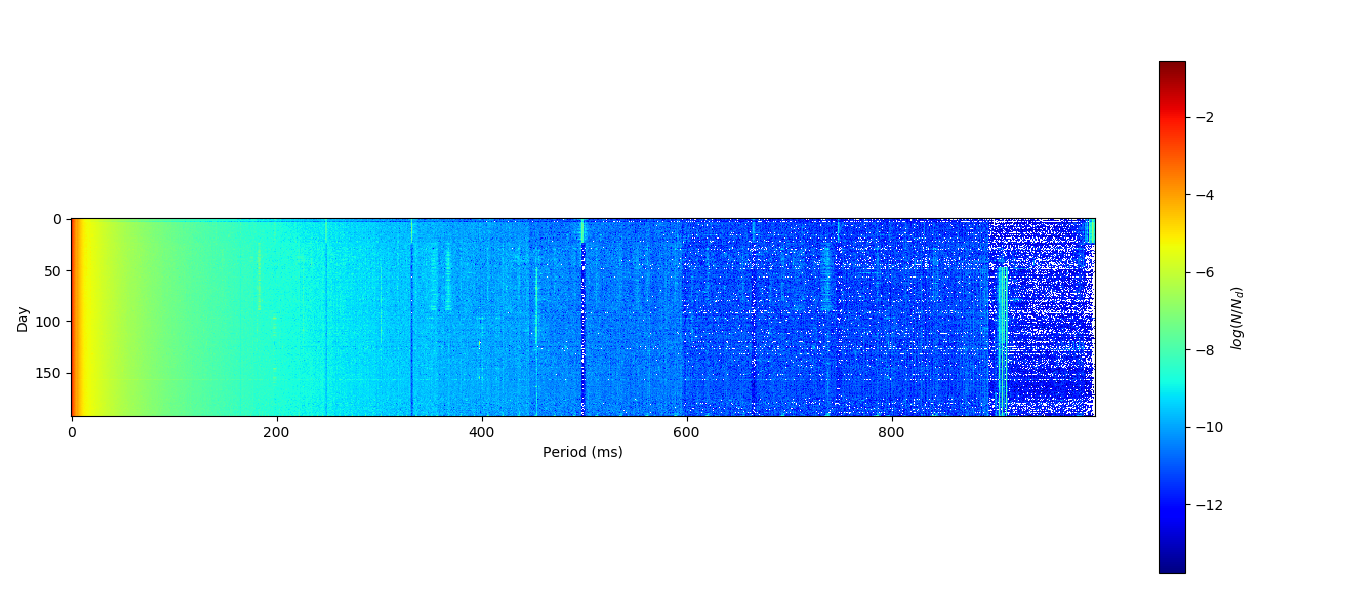
\includegraphics[width=1.0\textwidth]{figures/Full_log.png}
\caption{Distribution of the number of pulsar candidates with the detected period on each observation day. The data is normalised with the total number of candidates on the same day.}
\label{RFI_II}
\end{figure}


%\begin{figure}[h!] 
%\centering
%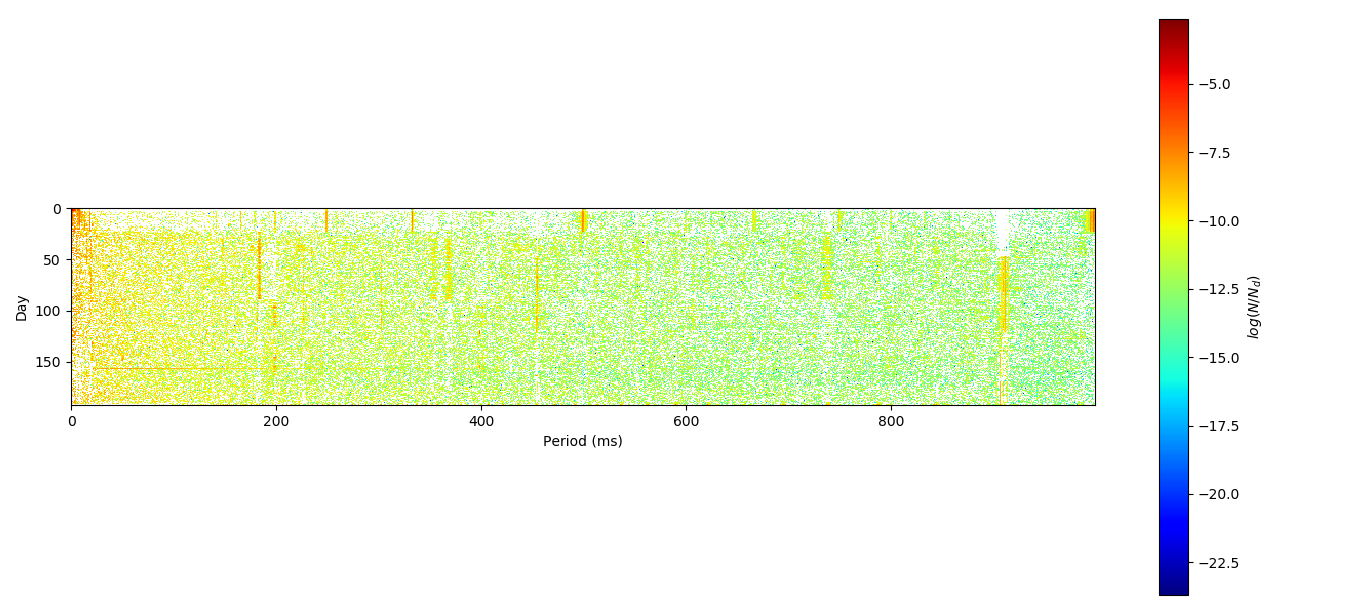
\includegraphics[width=1.0\textwidth]{figures/RFI_mit.png}
%\caption{The residual between \ref{RFI_II} and ``RFI profile'' }
%\label{RFI_I}
%\end{figure}

%\begin{figure}[h!] 
%\centering
%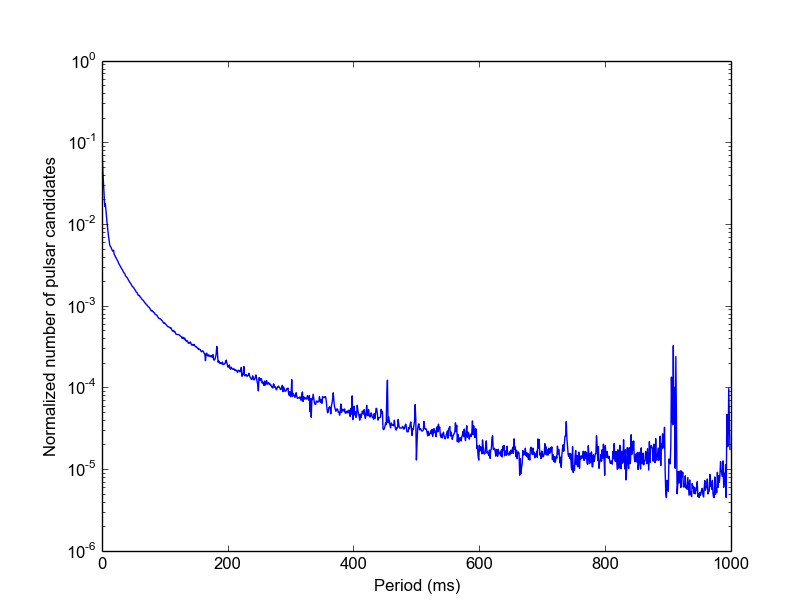
\includegraphics[width=0.7\textwidth]{figures/mean_profile.png}
%\caption{The "RFI profile" created from average normalised number of candidates from the whole observation campaign.}
%\label{RFI_profile}
%\end{figure}

        
        \subsection{De-dispersion} \label{DDM}
%        \paragraph{} Effect of DM, De-dispersion in theory, Type, step 
       % \paragraph{} As mentioned before, an effect of ISM will make a signal in each frequency arrive the Earth at a different time. This effect is removed by introducing a delay in each frequency as Equation \ref{delaytime}.
       \paragraph{} There are two ways of performing de-dispersion. The simplest way is the ``incoherent de-dispersion''. This method divides the total bandwidth into several channels and applies proper time shift estimated from Equation \ref{delaytime}, which is easy to apply and computationally inexpensive. However, this method is limited since each of the divided frequency band or ``sub-band'' retains some smearings. %The alternative method is called ``coherent de-dispersion'' (\citep{hankins1971microsecond} and \citep{hankins1975methods}) which is apply Fourier transformed (see more in Section \ref{FFT}) to the data and rotate the relative phase of each component Fourier spectrum by an amount that is proportional to the DM of the pulsar. Coherence de-dispersion is slower compared to the first method but be able to recover the original pulsar signal.      
       However, the DM for each pulsar is an unknown before the discovery. As a result, the data set needs to be ``de-dispersion'' in a different DM. 
        \paragraph{} To optimise the calculation time for the search pipeline, the dispersion step size needs to be optimised as well. We know that dispersion can reduce the S/N of the data by broadening the pulse profile. The apparent pulse width or effective pulse width for a top-hat pulse with an intrinsic pulse width of $W_{int}$ due to DM offset ($\Delta DM$) using sampling time $t_{samp}$ is explained by
        \begin{equation}
        W_{eff}=\sqrt[]{W_{int}^2+(8.3 \times 10^6 \times \frac{\Delta f}{f_c^3} \times |\Delta DM|)^2+t_{samp}},
        \end{equation}
 where $\Delta f$ is the bandwidth of this observation. The reduce in S/N by an offset of DM is estimated by 
        \begin{equation}
        S/N \propto \sqrt[]{\frac{P-W_{eff}}{W_{eff}}}.
        \end{equation}
        This relationship is shown in Figure \ref{DMcurve} and indicates that for long period or wide pulse width pulsar, the DM curve will be larger.       
                 \begin{figure}[h]
\centering
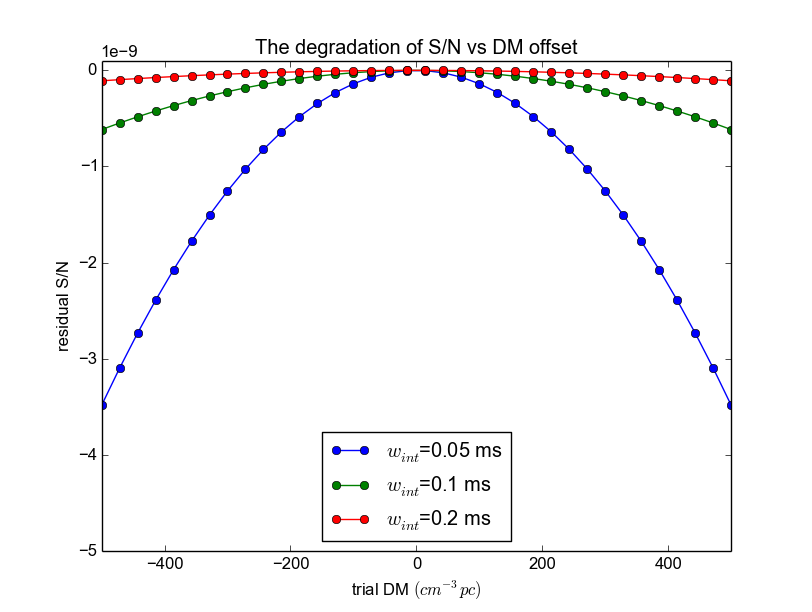
\includegraphics[width=0.80\textwidth]{figures/DMcurve-title.png}
\caption{Demonstration of Degradation of S/N by DM offset for  simulated 2s pulsar observed at $f_c= 430$ MHz and $\Delta f=$ 8 MHz.}
\label{DMcurve}
\end{figure}
        The dispersion step size is calculated by giving the condition that if the dispersion time is smaller than sampling time, the S/N will be the same. The $i^{th}$ DM value is written as 
        \begin{equation} \label{dm_step}
        DM_i=1.205\times10^{-7}  (i-1)t_{samp}(f_c^3/\Delta f) pc~cm^{-3},
        \end{equation}        
where $\Delta f$ is the total bandwidth in MHz. $f_c$ is the central frequency. At $i=n_{chan}+1$ or ``diagonal DM'', the dispersion delay across the bandwidth will be ``$n_{chan} \times t_{samp}$''. After the second diagonal DM is reached, the dispersion delay time on each channel becomes $2 t_{samp}$ , which allows us to ``down sampling'' the data by the factor of two. This process can be repeated when the DM gets higher to save the computational power. As a result, Equation \ref{dm_step} can be re-written as 
        
                \begin{equation} \label{dm_step_dig}
        DM_i=DM_{0}(i-1) Df,
        \end{equation}        
         
 where $DM_{1}$ is the first diagonal DM defined as $DM_0 = 1.205\times10^{-7} t_{samp}(f_c^3/\Delta f)pc~cm^{-3}$  and $Df$ is the down sampling factor. 

        
    \section{Algorithms for pulsar search}
    \paragraph{} After the data are de-dispersed, this data set needs to be ``searched" in order to see if there are any pulsar signals in that data set. In this section, three of pulsar search methods will be discussed.   
        	\subsection{Single pulse search (SP)} \label{SP}
        \paragraph{} The easiest way to search for a pulsar is to find any ``pulse'' that is strong enough in the time series. Imagine a time series with Gaussian noise. The ``pulse'' is detected by searching for any signal that is stronger than a certain standard deviation. In the best case where the pulse width is equal to sampling time ($t_{samp}$), \cite{cordes2003searches} shows that the S/N of the detected pulse is explained using
\begin{eqnarray}
S/N=\frac{S_{peak} W}{S_{sys}}\sqrt[]{\frac{n_p \Delta f}{W}},
\end{eqnarray}
where $S_{sys}$ is the system-noise equivalent flux density, $n_p$ is the number of polarisations, and $\Delta f$ is the bandwidth of the receiver. $W$ is the pulse width and $S_{peak}$ is the pulse amplitude. However, $W$ is not always equal to $t_{samp}$. Therefore, matched filtering algorithm needs to be applied to this time series. Matched filtering is down sampling the time series with different factor, searching for the factor that gives the best S/N . This is the factor where $W \sim t_{samp}$.

%\paragraph{} Single pulse search allows us to detect the pulsar that emits a strong pulse like giant pulse emitter. Giant pulse emitter is the pulsar which can produce a pulse that more than ten times stronger than the mean pulse intensity. 
    	\subsection{The Fast Fourier Transform (FFT)} \label{FFT}
%        \paragraph{}Principle, equation, application to pulsar search, missing population 
        \paragraph{} Another way to search for pulsar is to search for any periodicity in the time series. The most successful technique for pulsar search is to take the Fourier transform of the time series and study the Fourier frequency domain. However, since the time series is discrete, it is not possible to apply Fourier transform directly. The discrete Fourier transform (DFT) is used instead of discrete times series ($\mathcal{T}$) with N data point. The $k^{th}$ Fourier component of the DFT can be evaluated from        
 \begin{equation}
 \mathcal{F}_k=\sum_{j=1}^{N-1} \mathcal{T}_j exp(-2\pi ijk/N), 
 \end{equation}
 where k is the Fourier frequency and $i = \sqrt[]{-1}$. From Nyquist sampling theory, the range of frequency spectrum that can be obtained from DFT is $\frac{1}{t_{int}}<\nu<\frac{1}{2 t_{samp}}$ \citep{ransom2002fourier}. However, the DFT is relatively slow because it requires $N^2$ floating point operation. The faster version of the DFT is the fast Fourier transform (FFT) that requires $Nlog_2(N)$ operation. Imagine the time series with $10^6$ samples, the DFT needs $10^{12}$ operations while the FFT takes only $6log_2 10$, which is $10^5$ times faster than the former. The improvement of the FFT comes from the properties of the Fourier transform that can be written as $\mathcal{F}_{N-k}=(\mathcal{F}_k)*$, which makes the DFT symmetrical around $k=N/2$, which reduces the number of operation \citep{FFT}. A Fourier spectrum $\mathcal{P}_j$ is created from the summation between the real and imaginary parts of the Fourier components ($\mathcal{P}_k=|\mathcal{F}_k^2|$). The Fourier spectrum could be used to investigate the periodicity in time series as demonstrate in Figure \ref{FFT_im}.  
 
 \begin{figure}[h]
\centering
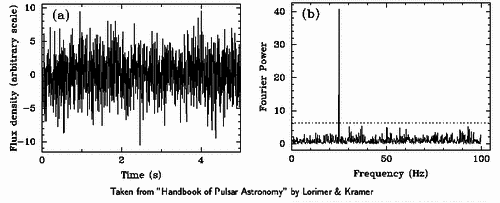
\includegraphics[width=0.80\textwidth]{figures/FFT}
\caption{Demonstration of applying the FFT to a time series with a 25 Hz periodic signal in the left side of the image. The result from the previous process is the power spectrum of this time series, showing a peak at 25 Hz as shown in the right image. The dashed line in the right image shows the detection threshold. Images are obtained from \citep{handbook}}
\label{FFT_im}
\end{figure}
\paragraph{} Unfortunately, the pulsed signal that we are searching for has a pulse width that could be a few percents of the period (0.2-25$\%$). This pulse width is also referred as ``duty circle'' $\delta$, which is the pulse width ($W$) divided by period (P) ( $\delta=W/P$). The time series with narrow pulses will result in the Fourier frequency spectrum in fundamental frequency and other harmonics. A technique is known as ``incoherent harmonic summing'' was implemented to pulsar search by \cite{taylor1969two} to maximise the detected S/N by adding lower harmonics to the fundamental spectrum as Figure \ref{FFT_ham}.

 \begin{figure}[h]
\centering
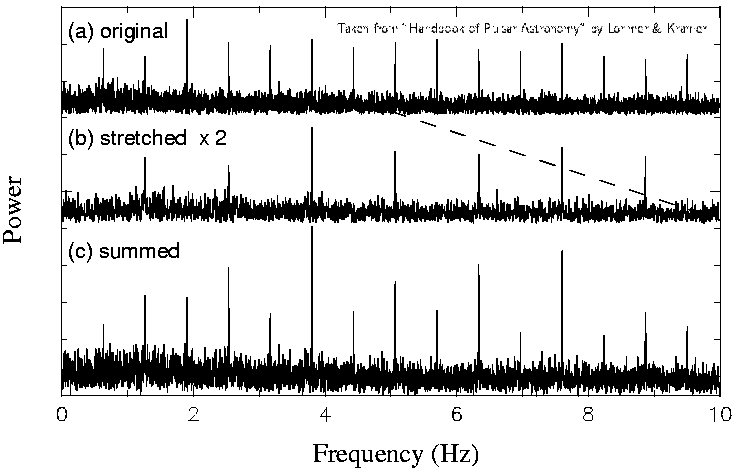
\includegraphics[width=0.8\textwidth]{figures/6_06.png}
\caption{Demonstration of the applying harmonic summing by stretching other half of the spectrum by a factor of 2 and adding that to the original spectrum. This process increases the S/N by a factor of $\sqrt[]{2}$. Repetition of this process will increase S/N by large factors. Images obtained from \citep{handbook}}
\label{FFT_ham}
\end{figure}
		%\paragraph{} To distinguish between real detection from random noise result, the significance of that signal needs to be determined. For a time series with Gaussian noise, \cite{handbook} shown that the minimum S/N of the signal that is real detection is 
        \paragraph{} For a time series with Gaussian noise, the minimum S/N for significant detection is shown by
        \begin{equation}
        S/N_{min}=\frac{\sqrt[]{ln[n_{trials}]}-\sqrt[]{\pi/4}}{1-\pi/4}.
        \end{equation}
		$n_{trials}$ is the total number of trial which is calculated from 
        \begin{equation} \label{n_trial}
        n_{trial}=N \times N_{dm} \times N_{acc}
        \end{equation}
 where $N_{dm}$  and $N_{acc}$is the total number of trial DM and acceleration respectively. The probability threshold for detecting random noise candidates is defined as ``False-alarm probability''. Details about this can be found at \cite{handbook}
\paragraph{} The FFT is one of the most successful algorithm for pulsar searches. However, the FFT have some limitations. For example, in searching for a long period pulsar (defined here as a pulsar which has a period longer than 1 s) as shown in  \cite{kondratiev2009new}. The alternative search algorithm will be discussed in Section \ref{FFA}. 

        \subsection{The Fast Folding Algorithm (FFA)} \label{FFA}
       % \paragraph{} Principle, equation, application on pulsar search  
        \paragraph{} An alternative way to search for periodicity in any time series is to directly fold de-disperse time series with different period and search for a significant pulse profile. However, brute-force folding algorithm needs $N[(N/n)-1]$ operations, where n is the number of profile bins. This process is computationally expensive in a similar way to the DFT. Shortly after an implementation of the FFT in 1965 \citep{FFT}, \cite{staelin1969passive} implemented the fast-folding algorithm (FFA). The FFA works by splitting a time series into a small fraction of n sample with the condition that $N/n$ is an integer power of 2, where N is the total sample number. These dived time series will be combined in a different way which represents different period, as shown in Figure \ref{FFA_im}. The folded profile p at $k^{th}$ bin is written as 
        \begin{equation}
        p_k=\sum_{j=0}^{N/P_0-1}\mathcal{T}_{k+jP_0},
        \end{equation}
        \paragraph{}The  FFA takes only $Nlog_2(N/n)$ operations. However, the FFA is still computationally expensive due to a high data sampling rate which makes the FFA not possible to apply to large survey before. FFA shows many advantages in searching for a slow pulsar. For example, even the slow pulsar has a pulse width of $1\%$. This pulse width is 10 ms (for 1 S pulsar). This means that the time series can be down sampling from the original $64 \mu s$ to $\sim 1ms$, which makes N $\sim 156$ times smaller. This smaller N leads to less operation. Moreover, the FFA gives a result in a fully coherent phase which can recover the sensitivity that is lost in FFT \citep{kondratiev2009new}. The result from FFA by varying $N/P_0$ will be displayed in a periodogram that shows S/N for each trial period. The searching plan for FFA is written as 
        \begin{equation}
        P_{max}=P_{min}+\frac{P_{min}}{bins_{min}} \times n_{bins},
        \end{equation}
where $bins_{min}$ is the minimum searching profile bins. $n_{bins} $ is the difference between maximum and minimum profile bins. A demonstration of thhe FFA search step is shown in Table \ref{FFA_step}. The sampling time for each period is selected from the fact that $t_{samp}$ for each period needs to be at least $\frac{1}{bins_{min}}$to create a pulse profile. This can introduce huge down sampling factor, $dfactor$. 
        
         \paragraph{} False alarm rate probability for the FFA is directly related to profile significance. The probability of detection pulse profile with specific S/N by random Gaussian noise is written as 
                 \begin{equation}
        Prob(>S/N)=\frac{1}{n_{trial}}=\frac{1}{\sqrt[]{2\pi}} \int^{\infty}_{S/N} e^{-x^2/2}=\frac{1}{2} [1-erf(\frac{S/N}{\sqrt[]{2}})].
        \end{equation}
        The error function $erf(x)$ could be solved numerically. For more information, see \cite{press1992numerical}. The number of trial in FFA is $n_{trial}=n_{FFA} \times N_{dm} \times N_{acc} $
         \begin{figure}[h]
\centering
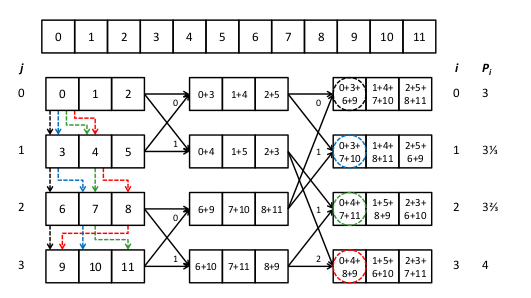
\includegraphics[width=0.80\textwidth]{figures/FFA.png}
\caption{Demonstration of applying the FFA to a time series with N=12. The time series is folded into 4 different trial periods. Each arrow represents the bin with the same color circle. Image obtained from  \cite{Andrew}}
\label{FFA_im}
\end{figure}
%		\paragraph{} The result from FFA by varying $N/P_0$ will be displayed in a periodogram that shows S/N for each trail period. 
        \subsection{Comparison between searching methods} \label{Com}
        \paragraph{} Investigating in each of search algorithm theoretical S/N is required in order to compare each of the search method. First, the single pulse search is basically a search for signal that exceeds the noise with matching filter. The S/N for a top hat pulse with flux $S$ and width $W$ in number of bins and the presence of noise with zero mean and standard deviation of unity are written as   
		\begin{equation}
		S/N_{SP}=S_{peak} \cdot \sqrt[]{W} \label{snr_sp}.
		\end{equation}       
        \paragraph{} The FFT is more complicated because it applies a harmonic summing to the data.\cite{kondratiev2009new} shows that $S/N_{FFT}$ for H harmonic sum is  
        		\begin{eqnarray}
		S/N_{FFT}=\sqrt[]{\frac{\pi}{H(4-\pi)}} \sum^H_{n=1}[L^0_{1/2}(-N[S_{av}(1-\delta)sinc[\pi n (1-\delta)]]^2)-1] \label{snr_fft},
		\end{eqnarray}    
where $L^0_{1/2}(x)$ is the generalised Laguerre polynomial $L^{\alpha}_{n}(x)$.  $S_{av}$ is the average pulse flux over the integration time  %which depends on pulse flux distribution. 
        $\delta$ is the ``duty circle ($\delta$)'' defined by $\delta=w/P$
        \paragraph{} The FFA is similar to SP but FFA is to detect average pulse profile that integrates over a number of pulses ($N_p$).  \cite{kondratiev2009new} proposed that S/N for FFA is written as
        \begin{equation}
		S/N_{FFA}=S_{av} \cdot \sqrt[]{W} \cdot \sqrt[]{N_p}. \label{snr_ffa}
		\end{equation}
	\paragraph{} The comparison between FFA and FFT has been done by \cite{Andrew} and \cite{kondratiev2009new} as shown in Figure \ref{FFA_FFT_com}. This comparison shows the advantage of FFA to FFT in searching for long period and narrow pulse width pulsar.  Dividing Equation  \ref{snr_ffa} with Equation \ref{snr_sp} gives 
    \begin{equation} \label{r}
    \frac{S/N_{FFA}}{S/N_{SP}}=\frac{S_{av} \sqrt[]{N_p}}{S_{peak}}.
    \end{equation}
    
\begin{figure}[h] \centering
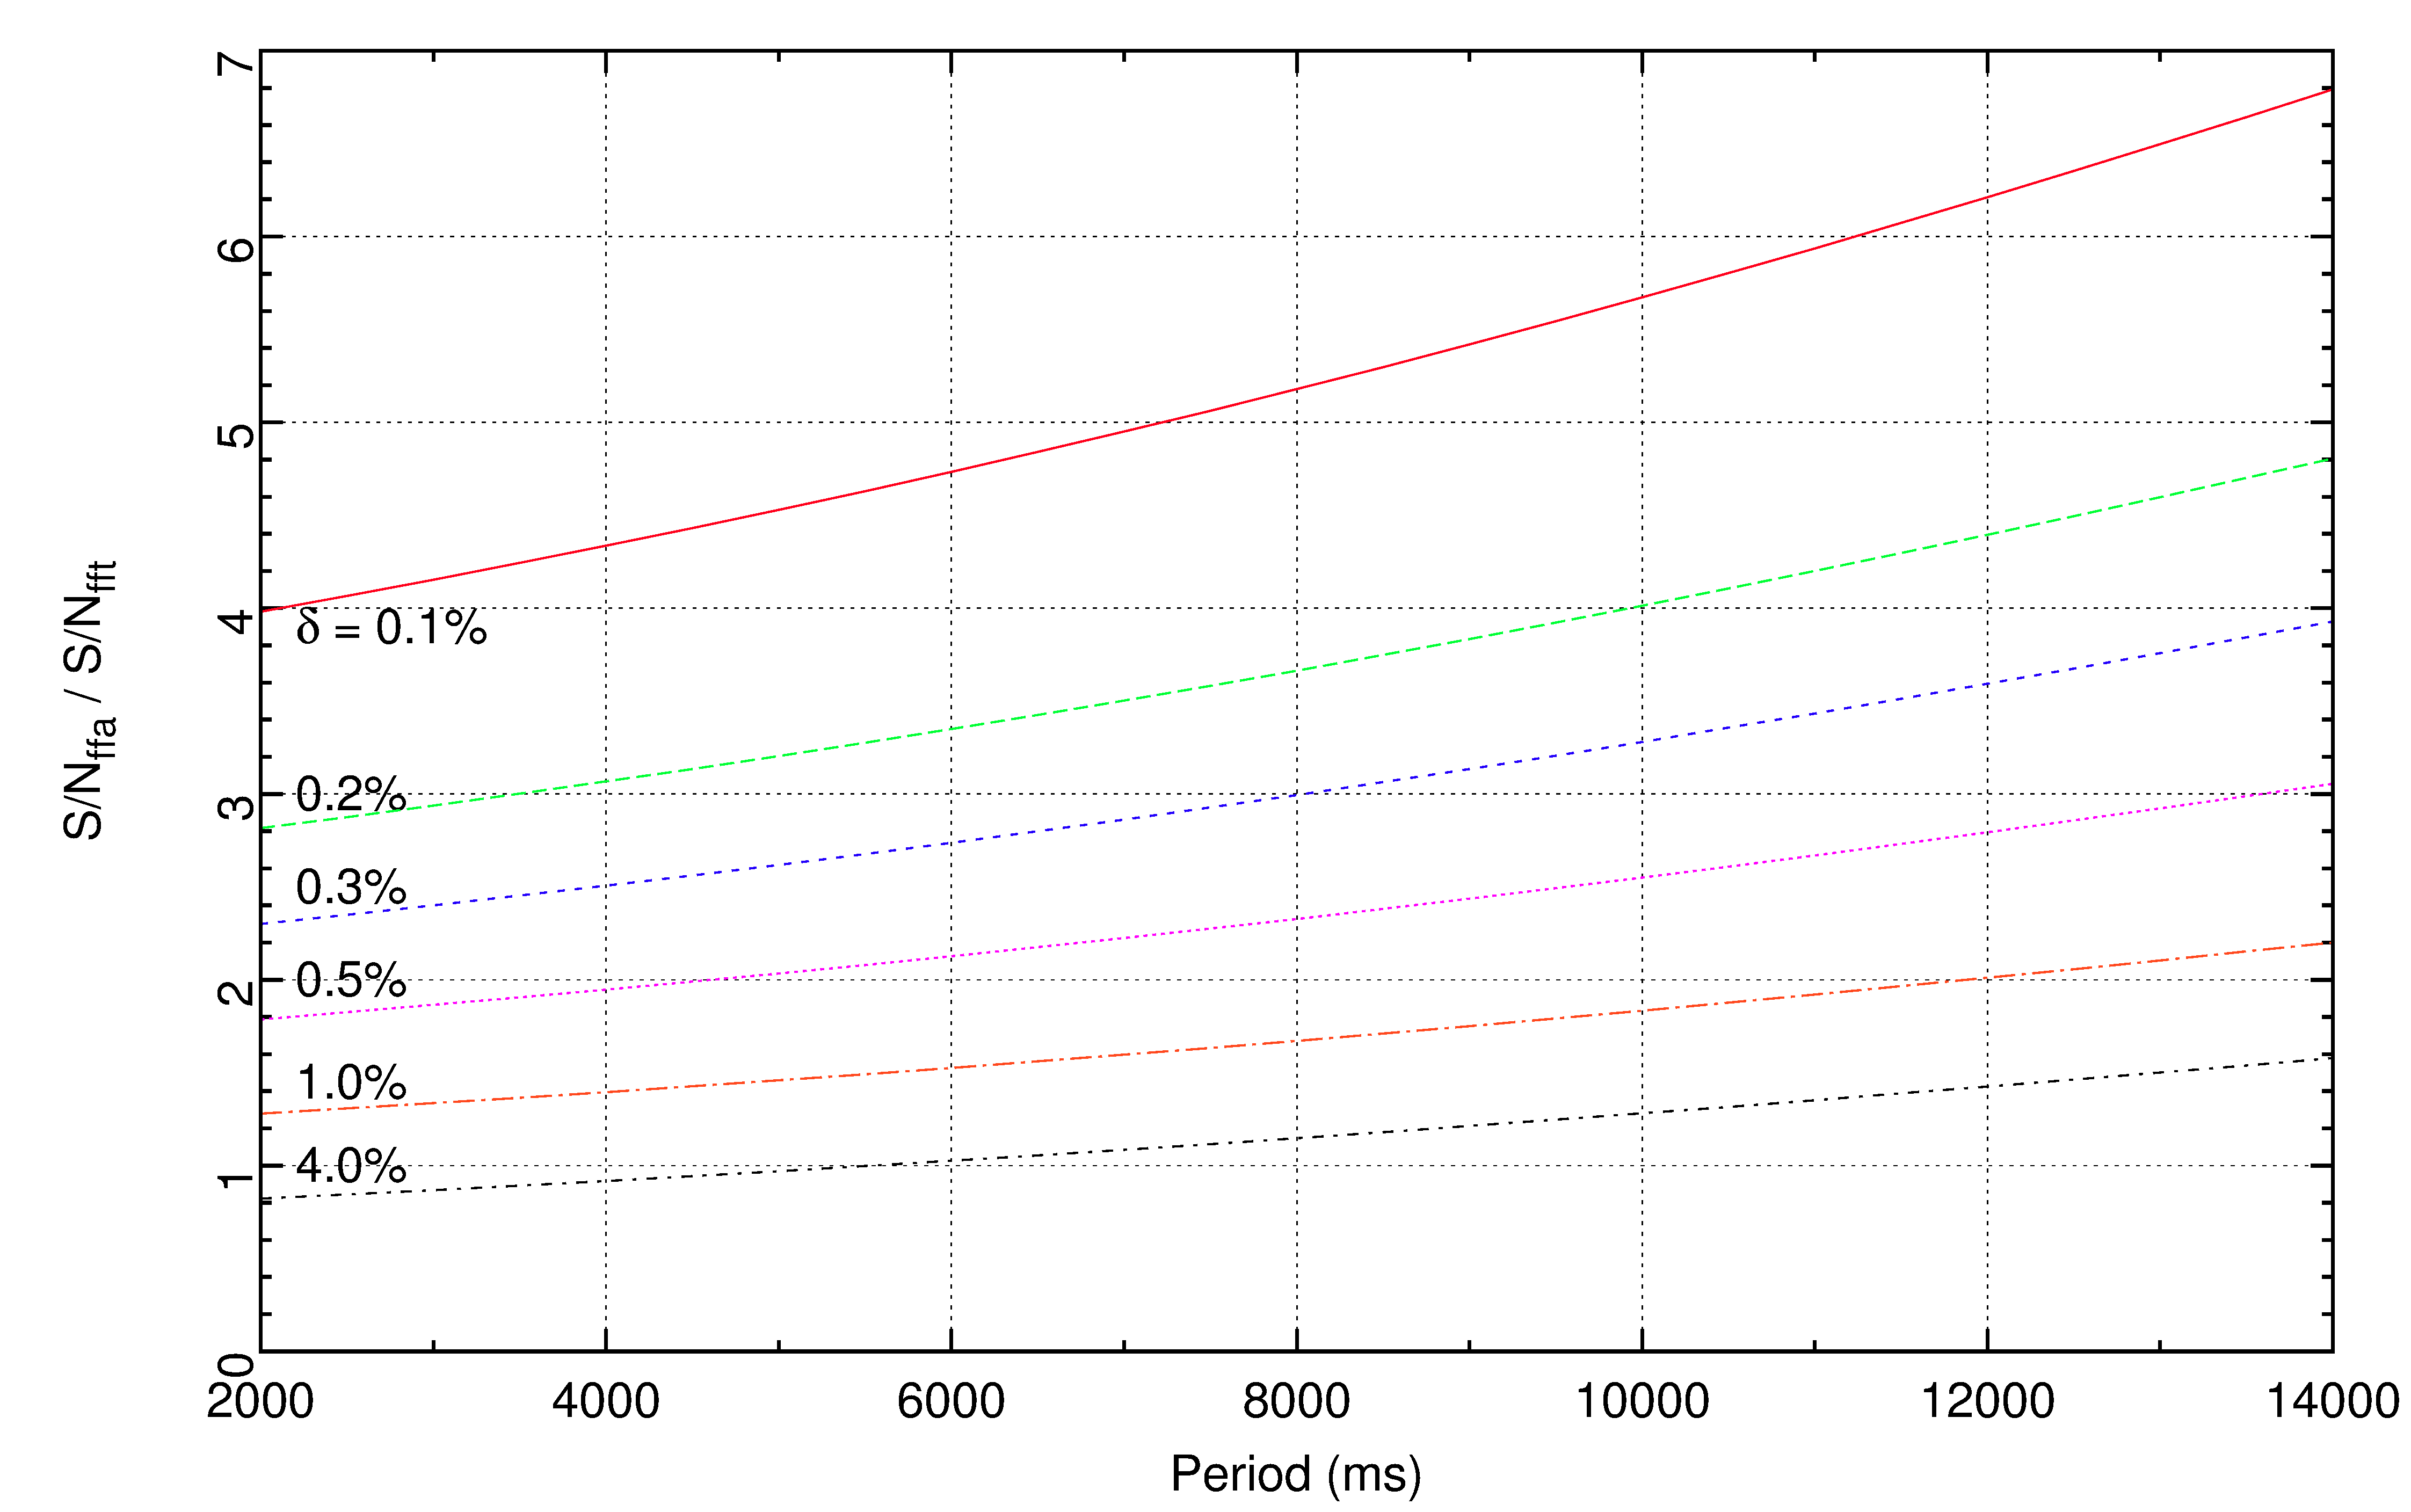
\includegraphics[width=0.80\textwidth]{figures/FFA_FFT.png}
\caption{The analytical prediction of the ration between $S/N_{FFA}$ to $S/N_{FFT}$ as a function of period and duty circle. Image by ~\cite{Andrew}}
\label{FFA_FFT_com}
\end{figure}

	\paragraph{} \cite{keane2011transient} and \cite{mclaughlin2003searches} attempted to compare SP with other algorithms with ``lognornal'' pulse flux distribution. This is typically observed from normal pulsar (\cite{cairns2001intrinsic}, \cite{johnston2001high}, and \cite{serylak2009simultaneous}) while pulsar emits ``giant pulses'', which are pulses that more than 10 times stronger than average flux \citep{karuppusamy2010giant}. The pulse flux distribution for this type of pulses is well described by power laws. 
    \paragraph{} For the lognormal distribution, the flux (S) distribution ($f(S)$) is described as 
    \begin{equation}
    f(s)=\frac{1}{\sigma \sqrt[]{2 \pi}} \frac{exp(-\frac{(ln S - \mu)^2}{2 \sigma^2})}{S}    \end{equation}
    Moreover, the peak flux ($S_{peak}$) and average flux are written as 
    \begin{eqnarray}
     S_{peak}=exp(\sqrt[]{2} ~ erfinv(1-\frac{2}{N})+\mu) \label{Speaklog}\\
    S_{av}=\frac{1}{2} exp(\mu+\frac{1}{2} \sigma^2) (1+erf(\frac{1}{\sigma \sqrt[]{2}} (ln S_{speak} - \mu)-\sigma^2)) \label{Savlog}
    \end{eqnarray}
   
where $erfinv(x)$ \footnote{see more https://docs.scipy.org/doc/scipy/reference/generated/scipy.special.erfinv.html} is inverse error function which can be solved numerically. \cite{cairns2001intrinsic} have evaluate $\mu =2.3$ and $\sigma = 0.096$ for the Vela pulsar. % \cite{weltevrede2006bright} also determined $\mu = 0.34$ and $\sigma = 0.99$ for lognormal model of PSR B0656+14. 
   
   \paragraph{} For Power-laws distribution, the distribution is given as 
\begin{equation}
f(S)=AS^{-\alpha} \label{fpower}
\end{equation}
    For this type of pulses, they are assumed to emit in a finite range between $S_1$ and $S_2$. The peak flux density is written as
  \begin{equation}
  S_{peak}=\left\{
    \begin{array}{@{}ll@{}}
    [(\frac{N-1}{N})S_2^{1-\alpha}+\frac{S^{1-\alpha}_1}{N})]^{\frac{1}{1-\alpha}}, & \ \alpha \neq 1 \\ \\
    S_1(\frac{S_2}{S_1})^{\frac{N-1}{N}}, & \ \alpha = 1
  \end{array}\right. \label{Speakpo}
  \end{equation}
and the average flux is written as
  \begin{equation}
  S_{av}=\left\{
    \begin{array}{@{}ll@{}}
    (\frac{\alpha-1}{\alpha-2})(\frac{x^{\alpha-2}-1}{x^{\alpha-1}-1}) S_{peak}, & \ \alpha \neq 1,2 \\ \\
    \frac{S_{peak}-S_1}{ln(S_{peak}/S_1)}, & \ \alpha = 1 \\ \\
    \frac{S_1 ln x}{S-S_1} S_{peak}, & \ \alpha = 2,
  \end{array}\right.
  \end{equation}
  where $x = \frac{S_{peak}}{S_1}$, derived from Equation \ref{x} , is written as 
   \begin{equation}
  x=\left\{
    \begin{array}{@{}ll@{}}
    [(\frac{N-1}{N})+\frac{1}{N}(\frac{S_2}{S_1})^{\alpha-1}]^{\frac{1}{1-\alpha}} (\frac{S_2}{S_1}), & \ \alpha \neq 1 \\ \\
    (\frac{S_2}{S_1})^{\frac{N-1}{N}}., & \ \alpha = 1.
  \end{array}\right. \label{x}
  \end{equation}This equation is used to calculate analytic S/N ratio from the FFA and the FFT.   
  \paragraph{} The comparison between the FFA and the FFT is shown in Figure \ref{FFA_SP_com}. This shows that normal pulsars are likely to be detected using the FFA than SP search.  The condition that makes SP more effective that FFA is when there are less than 3 pulses in the whole observation. For an integration time of 4320s, the integration time for the survey used in this work, the pulse period of 3 pulses for the whole observation is 24 minutes, which is extremely longer than the longest period pulsar \footnote{The longest period pulsar found in October 2018 is 23.5s \cite{tan2018lofar} }.  For giant pulse emitter, \cite{keane2011transient} demonstrated that SP is more effective for giant pulse emitter with flux distribution that follows power laws, given that $1<\alpha<3$.  The result from Figure \ref{FFA_SP_com} ais in line with this assumption.  
  
  \paragraph{} This means that the FFA is useful in searching for a slow ($P>1~s$ ) and wide pulse width pulsar while the FFT is adequate for the fast spinning pulsar. Moreover, SP is not useful in order to search for the ordinary pulsar in long integration time because as the integration time gets longer, the number of pulses increases with $S/N_{FFA}$.  SP becomes more effective when we are searching for giant pulse emitter pulsar, as shown in Equation \ref{r}.  Giant pulse emitter an emitted pulse that is 1000 times brighter than average flux \citep{karuppusamy2010giant}.  This means that the ratio between $S_{av}$ and $S_{peak}$ is lower for this type of pulsar, leading to more efficiency in SP. 


  \begin{figure}[h] \centering
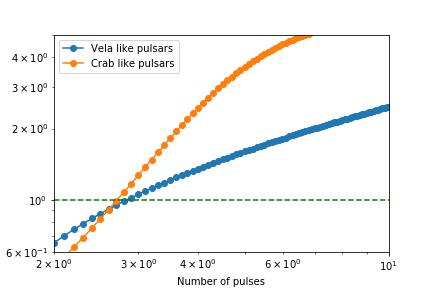
\includegraphics[width=0.80\textwidth]{figures/FFA_SP}
\caption{The analytical prediction of the ratio between $S/N_{FFA}$ to $S/N_{sp}$ as a function of period.  The giant pulse emitter or the Crab like pulsar is defined using a power law flux distribution of $\alpha$=3. The normal pulsars are noted as Vela pulsars.}
\label{FFA_SP_com}
\end{figure}
  
    \section{Binary pulsar search} \label{BS}
%	\paragraph{} Effect on binary motion to pulsar signal, time domain re sampling, acceleration search and 10 percent rule.   
	\paragraph{} Being in a binary system could change the apparent period of a pulsar. Altering the period could transfer the emitting power to other spectrum/periodogram bins, which  reduces the S/N ratio. One of the ways to recover this signal is using the technique called ``time domain resampling''. Time domain resampling is a technique to resample the time series into the rest frame of the pulsar. The core of this process begins with the relation between pulsar time interval $\tau_0$  as a moving emitter with velocity $V_1(t)$ and observer time interval $\tau$; 
\begin{equation}
\tau=\tau_0(1+V_1(t)/c)
\end{equation}
$c$ is the speed of light. If we assume that the acceleration ($a$) along the observation time is constant ($V_1(t)=at_{obs}^2$), the equation above can be re-written as 
\begin{eqnarray}
\tau=\tau_0(1+\frac{at}{c})
\end{eqnarray} 
In this work, I will focus on applying acceleration search to the FFA for the first time.

\paragraph{} We can search for pulsar with a constant acceleration by applying the time domain resampling with different acceleration trails ($\delta a$). To calculate an optimal step size for acceleration trials for observation time $t_{int}$, the period in observer frame ($P$) needs to change less than one pulse profile bin. The explanation of this method is similar to diagonal DM, as explained in Section \ref{DDM}. The only situation where the signal can be lost from FFA is when the smearing time is more than a bin, as shown in Figure \ref{diag}. In this work, I choose the pulse profile bin to be 1/128 of the trial period (P). Moreover, we can see that the relationship between $\tau$ and $\tau_0$ is quadratic. As a result, the re-sampling time will be calculated from the middle of the observation ($t_{obs}/2$)to minimise this effect. The acceleration step can be calculated using
\begin{eqnarray}
t_{samp}=\frac{\delta at^2}{2c}\\
a_0 = \frac{8c t_{samp}}{(t_{obs}/2)^2}\\
a_0 = \frac{8c t_{samp}}{2 t_{obs}^2}\\
a_i=a_0(i-1)Df \label{acc_step}
\end{eqnarray}
The testing result from this implementation could be found in Section \ref{AFFA}. From Equation \ref{acc_step}, I found that the FFA has a potential for further optimisation by making acceleration step for each trial period as if the $Df$ increases especially for the FFA search. Further detairegardils ng the acceleration with the FFA is discussed in Chapter \ref{Chapter:FFA_c}. The ``constant acceleration assumption'' has to follow the condition that the observation time ($t_{obs}$) needs to be less than $10\%$ of the the orbital period $P_{orb}$ \citep{ransom2002fourier}.

\paragraph{} The acceleration range can be calculated from Kepler's third law assuming that the orbital inclination is equal to $90^o$. The maximum acceleration magnitude is written as
\begin{equation}
|a_{max}|=(\frac{2\pi}{P_{orb}})^{\frac{4}{3}}(T_\odot f)^{\frac{1}{3}}c, 
\end{equation}
where c is the speed of light and $T_\odot=GM_{\odot}/c^3$. The mass function $f_m$ is 
\begin{equation}
f_m=\frac{m_c^3}{(m_p+m_c)^2},
\end{equation}
where $m_p$ is the mass of the pulsar assumed to be $1.4M_\odot$ and $m_c$ is the companion mass (see more at \cite{ng2015high}). 



    \section{Candidate selections} \label{Section:candidate_selection}
   % \paragraph{} Whats difference between Pulsar and RFI ? 
    \paragraph{} After all the steps above, the pulsar in the search range should be detected with significant S/N in multiple harmonics, DM, and acceleration. Therefore, the `candidate sifting' is required to identify if that candidate belongs to the same pulsar/RFI. The ``sifting'' is grouping up all the harmonically related candidates and find the best S/N candidate. All of the data will be plotted into many plots for each candidate, called ``diagnosis plot''. Examples of RFI and pulsar candidates are shown in Figure \ref{J1745_p} and \ref{RFI_p} respectively. The first column from the left side of the figures shows important numbers of this candidate. The next column shows the phase-time plot, integrated profile, and the relation between S/N and pulse profile. The last column illustrates the relationship between S/N with DM, period, and acceleration at that DM and Period. This ``diagnosis plot'' is modified by an FFA package, called ``riptide,'' with some modification of acceleration search. The detailed about ``riptide'' will be mention in Chapter \ref{Chapter:FFA_c}
    \begin{figure}[h] \centering
    \subfigure[An example of a pulsar candidate. ]
    {
    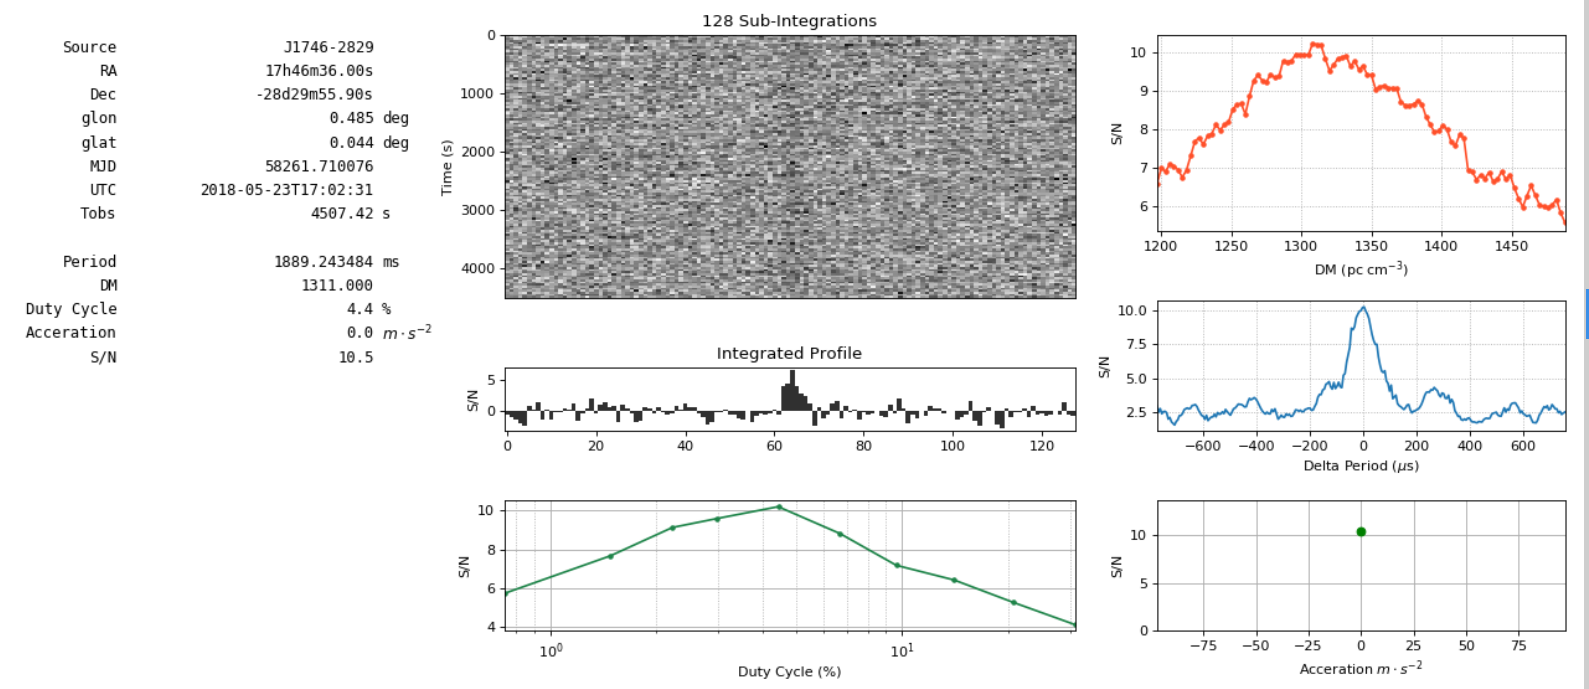
\includegraphics[width=1.0\textwidth]{figures/J1746-2829.png} 
    \label{J1745_p}
    }
	 \subfigure[An example of a strong periodic RFI showing low DM. Moreover, this candidate has a sinusoidal profile which is the signature of human-made RFI. ]
    {
    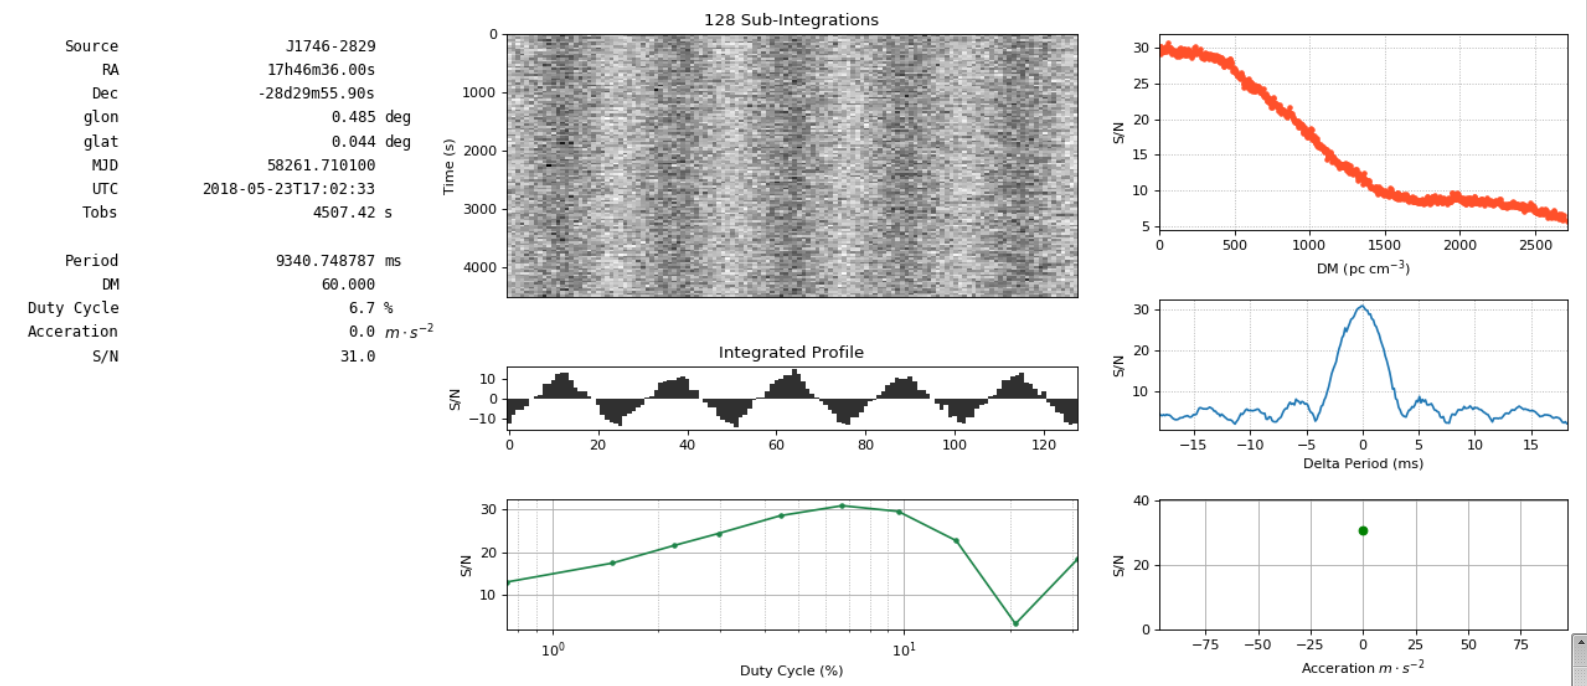
\includegraphics[width=1.0\textwidth]{figures/RFIP.png}
    \label{RFI_p}
    }
\end{figure}
	

    
\end{document}